\chapter{INSTRUKCJA UŻYTKOWANIA}
\label{chapter:instrukcja_uzytkowania}

\section{Opis dostępnych widoków}

\subsection{Strona tytułowa}


Strona tytułowa aplikacji pełni funkcję ekranu startowego, witając odbiorcę logiem oraz hasłem zachęcającym do korzystania z aplikacji. Widnieje na niej przycisk \textit{Get Started}, który umożliwia przejście do kolejnych widoków. Jeśli eksploatator był zalogowany w ciągu ostatnich 7 dni, aplikacja przekierowuje go do widoku logowania. W przeciwnym wypadku trafia on do ekranu profilu. 

\begin{center} 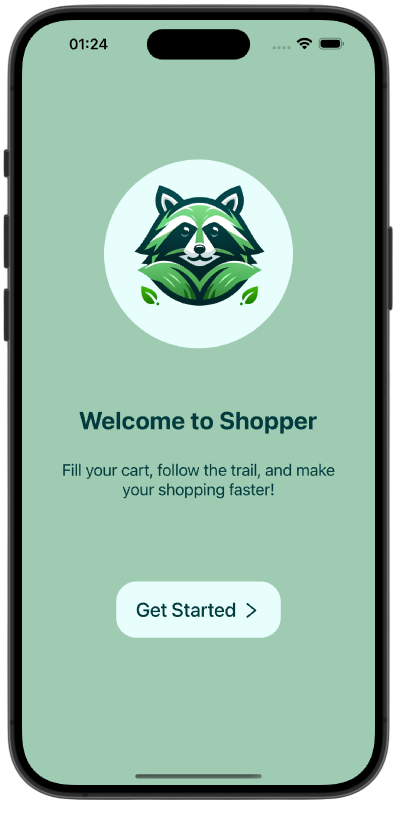
\includegraphics[width=0.3\textwidth]{images/front/home_page.png} \end{center}

Całość utrzymana jest w przyjaznej stylistyce, z dominującym odcieniem zieleni oraz spójną paletą kolorów, wygenerowaną przez narzędzie DALL·E 3 od OpenAI.

\begin{center} 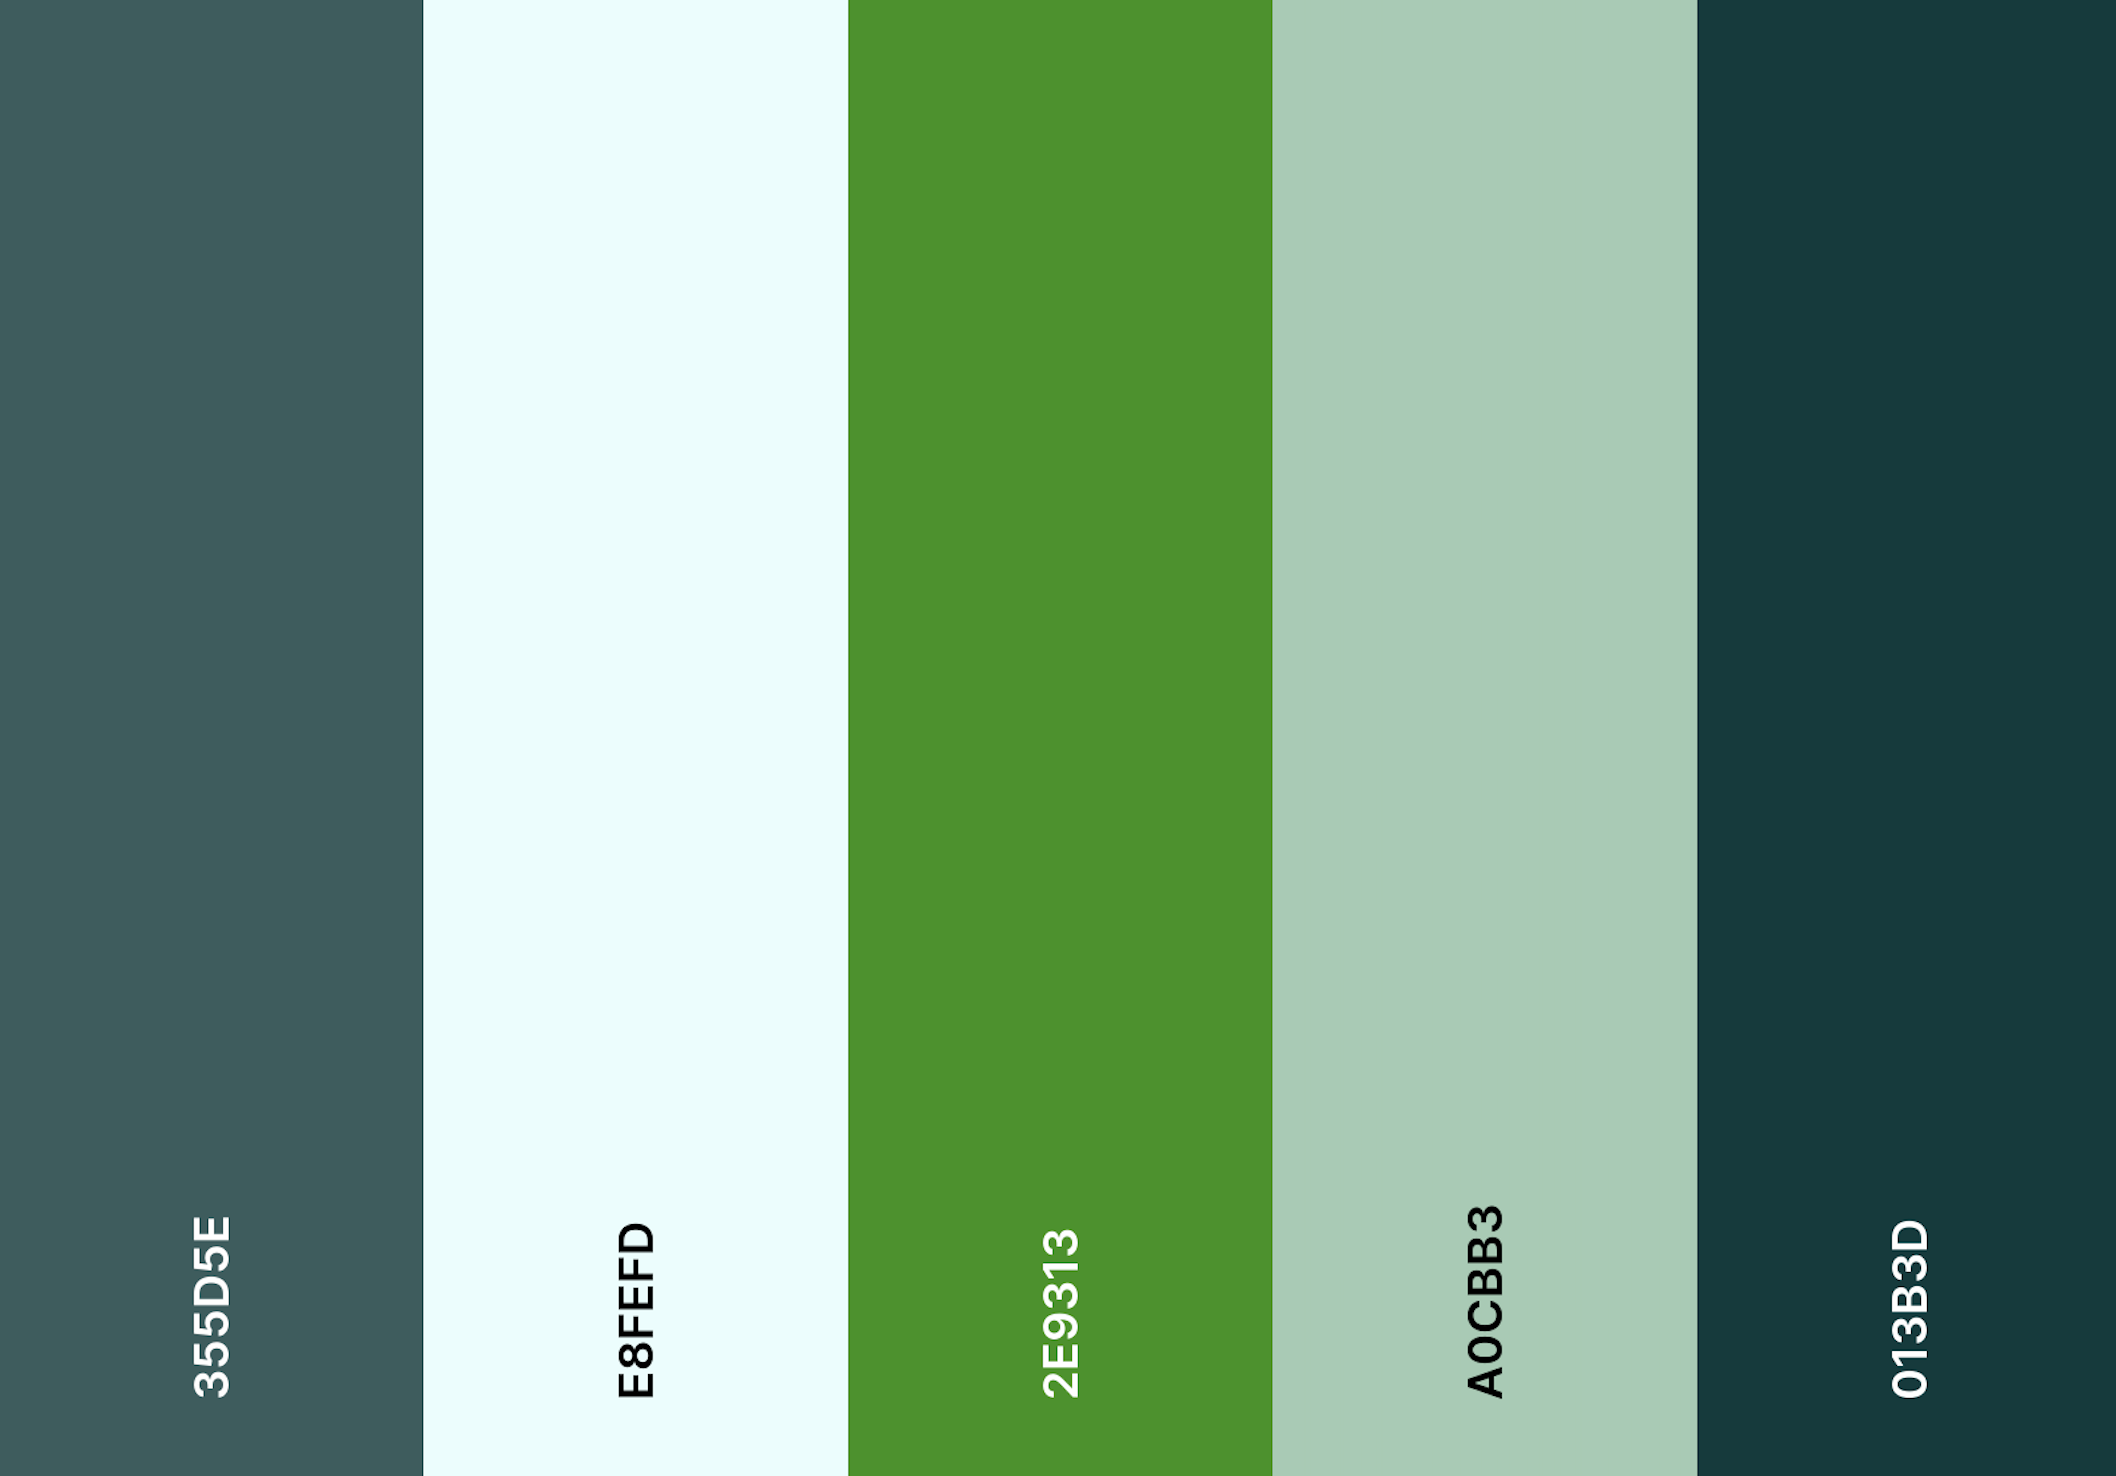
\includegraphics[width=0.3\textwidth]{images/front/theme.png} \end{center}

\subsection{Ekran logowania}

Ekran logowania umożliwia odbiorcy uwierzytelnienie w aplikacji, poprzez wprowadzenie adresu e-mail oraz hasła. Jego głównym celem jest weryfikacja tożsamości eksploatatora oraz przekierowanie do dalszych widoków w zależności od wyniku logowania. 

\begin{center} 
    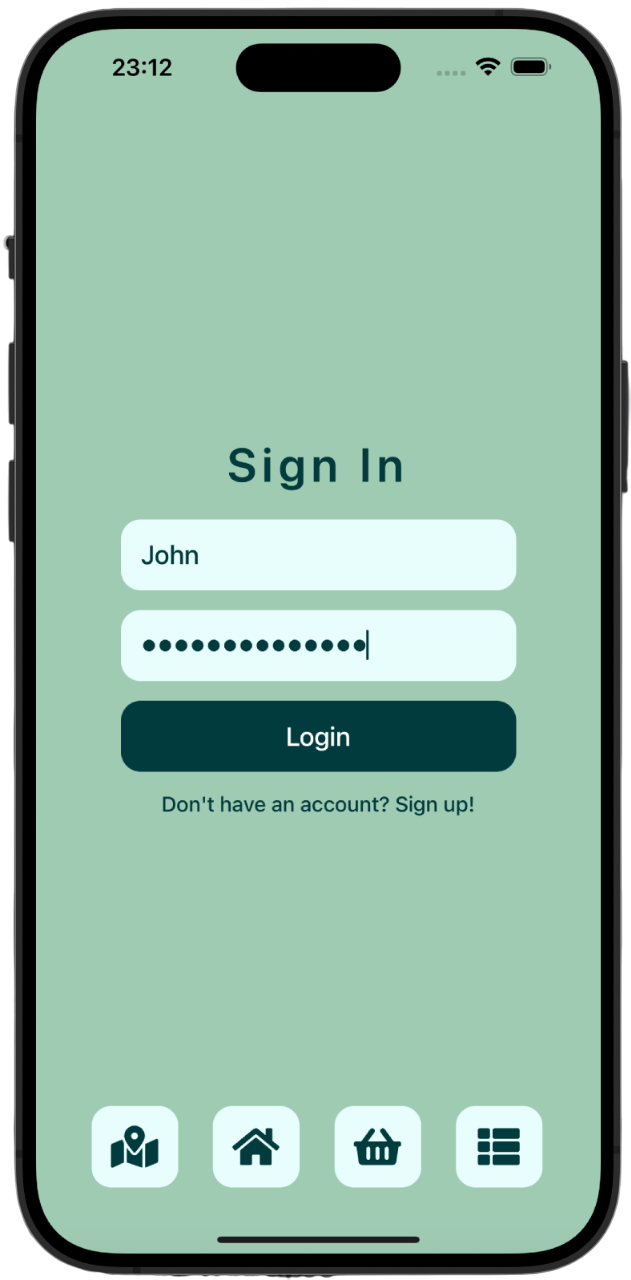
\includegraphics[width=0.3\textwidth]{images/front/login_page.png} 
\end{center}

Górną część widoku stanowi nagłówek \textit{Sign In}, który podkreśla cel ekranu. Tuż pod nim znajduje się formularz składający się z dwóch pól tekstowych: jednego przeznaczonego do wprowadzania adresu e-mail, a drugiego do hasła, z cechą ukrywania wprowadzanych znaków. Naciśnięcie przycisku \textit{Login} uruchamia logikę, która weryfikuje tożsamość odbiorcy na podstawie danych wprowadzonych w polach tekstowych. W przypadku niepowodzenia gość otrzymuje odpowiedni komunikat, informujący o niepoprawnym e-mailu lub haśle. Dla nowych kupujących, widok zapewnia przejście do ekranu rejestracji, poprzez kliknięcie w link \textit{Don't have an account? Sign up!}. 

Dolną część ekranu zajmuje pasek nawigacyjny z ikonami, które przenoszą do kolejnych podstron: mapy sklepów, profilu odbiorcy, kategorii produktów wybranego sklepu oraz strony tytułowej. Tylko ta ostatnia jest dostępna dla niezalogowanych użytkowników.

\begin{center} 
    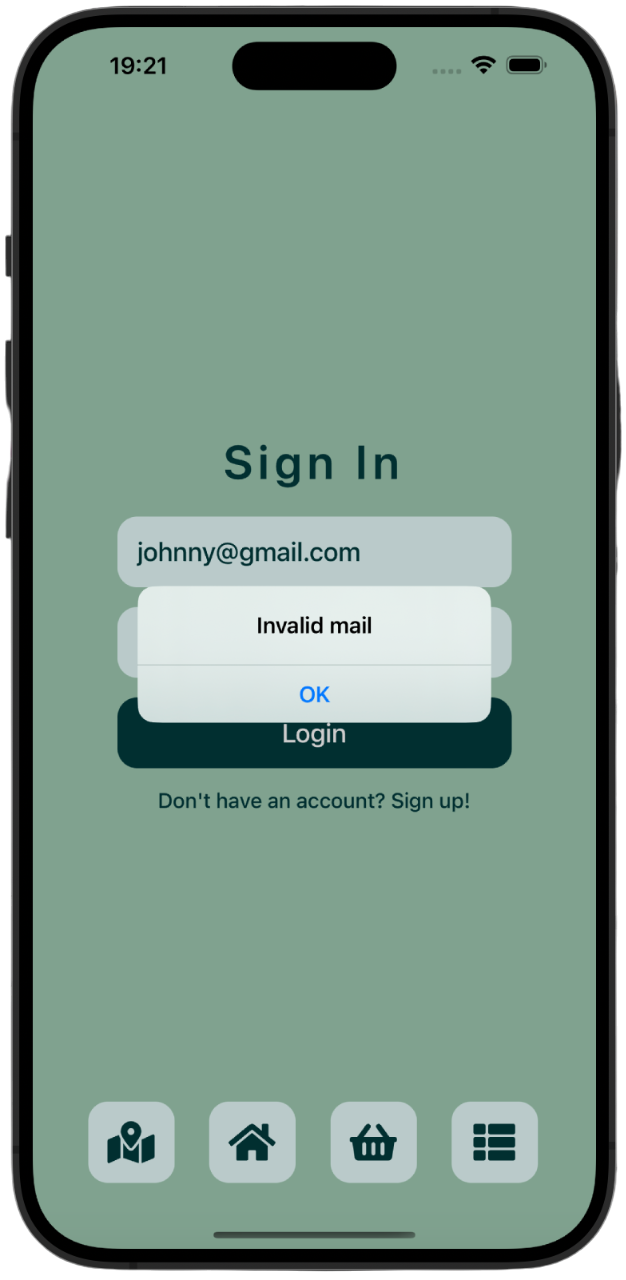
\includegraphics[width=0.3\textwidth]{images/front/login_invalid.png} 
    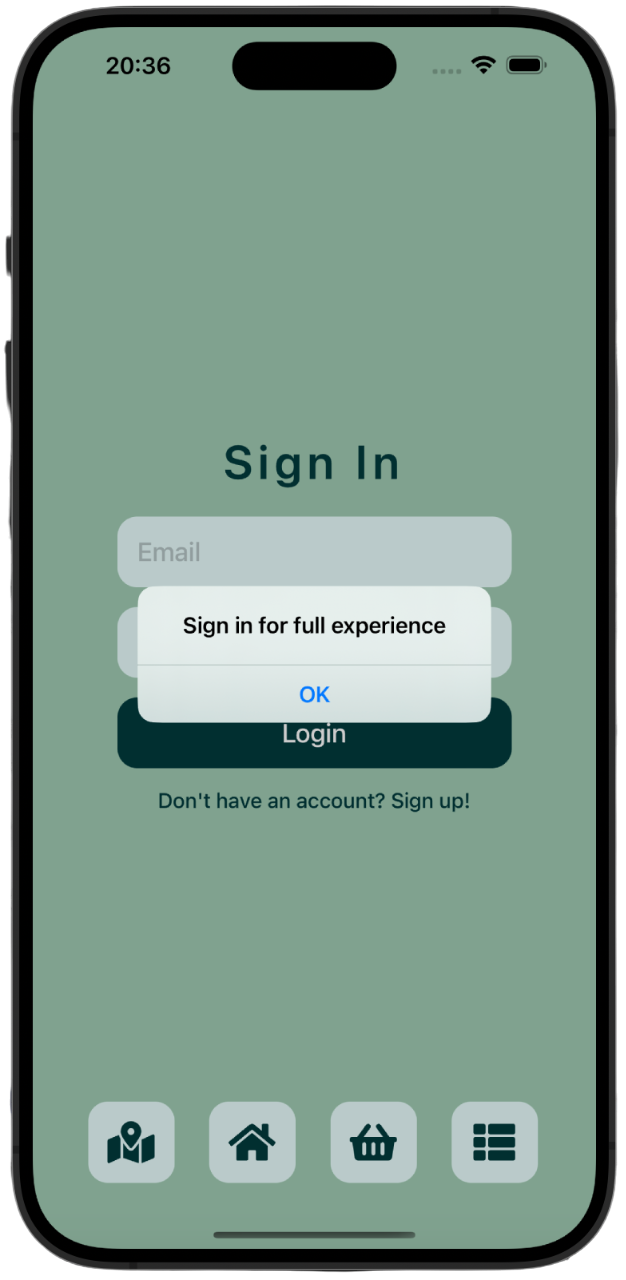
\includegraphics[width=0.3\textwidth]{images/front/login_not_signed.png} 
\end{center}

\subsection{Rejestracja użytkownika}

Ekran rejestracji umożliwia nowym odbiorcom założenie konta, co jest niezbędne do korzystania z funkcji wymagających uwierzytelnienia, takich jak dodawanie produktów do koszyka czy przeglądanie sklepów na mapie. Formularz rejestracyjny składa się z kilku pól:
\begin{itemize} \item \textit{Firstname} i \textit{Lastname} – wymagane minimum trzech znaków, by dane były wystarczająco szczegółowe. \item \textit{Email} – odbiorca podaje swój adres e-mail, który jest weryfikowany pod kątem poprawności formatu (obecność znaku \textit{@} oraz domeny). \item \textit{Password} i \textit{Repeat password} – hasło musi mieć co najmniej osiem znaków i być identyczne w obu polach. Dodatkowo, tekst wprowadzony w tych polach jest ukrywany, aby zapewnić prywatność. \end{itemize}

\begin{center} 
    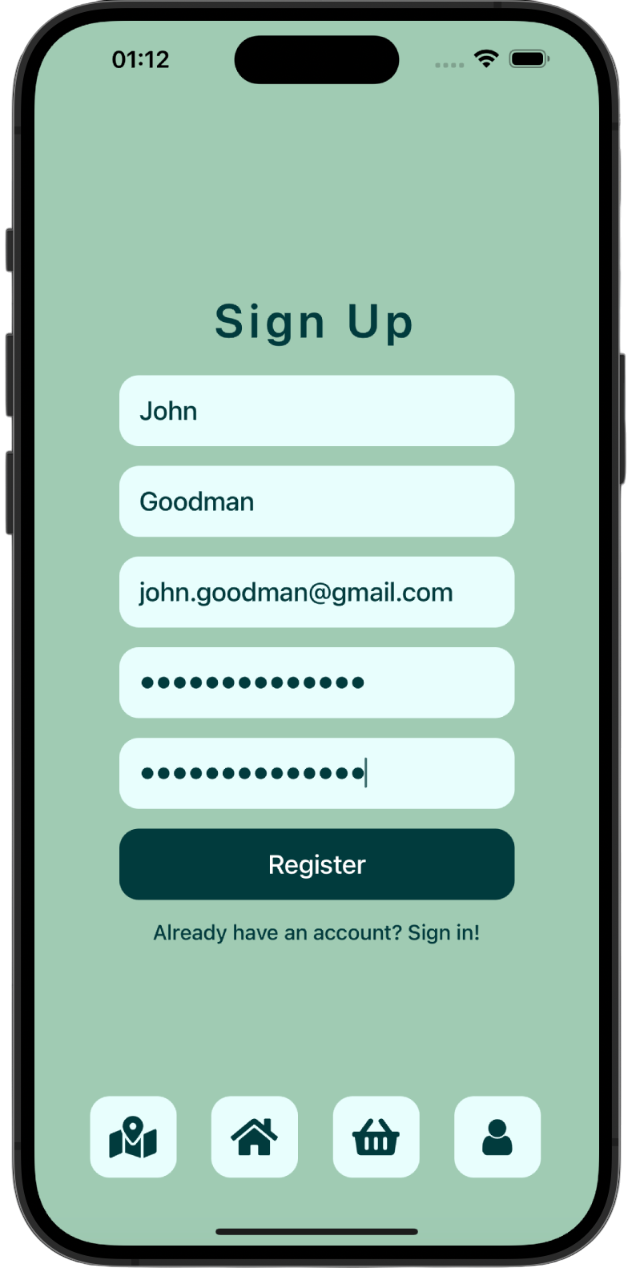
\includegraphics[width=0.3\textwidth]{images/front/register_page.png}
\end{center}

Po wypełnieniu formularza, należy wcisnąć guzik \textit{Register}, po którym odbywa się walidacja danych. W przypadku spełnienia warunków wpisanych pól, nowy użytkownik, wraz z koszykiem jest rejestrowany w bazie danych. Po zakończeniu rejestracji następuje automatyczne zalogowanie, a imię oraz ID są zapisywane w lokalnej pamięci urządzenia, w bezpieczny sposób, aby dane nie trafiły w niepowołane ręce. Pozwala to na sprawne obslużenie mechanizmu sesji oraz dostępu do koszyka jego właściciela. Następuje po tym przekierowanie do ekranu kategorii produktów wybranego sklepu. Jeśli dane są nieprawidłowe, wyświetlane są stosowne komunikaty, informujące o błędach, takich jak niewłaściwy format e-maila, zbyt krótkie hasło czy jego niezgodność. Osoby posiadające już konto mogą skorzystać z linku \textit{Already have an account? Sign in!}, znajdującego się pod formularzem, aby przejść do ekranu logowania. 

Dolną część ekranu zajmuje pasek nawigacyjny, który zawiera przyciski prowadzące do kolejnych sekcji aplikacji. Pierwszy z nich przekierowuje do widoku mapy sklepów. Kolejny przekierowuje na stronę główną – jest to jedyny dostępny dla niezalogowanych odbiorców. Trzeci zawiera ikonę koszyka, w którym użytkownicy mogą przeglądać swoje produkty, a czwarty prowadzi do profilu odbiorcy, gdzie można zarządzać danymi konta.

\begin{center} 
    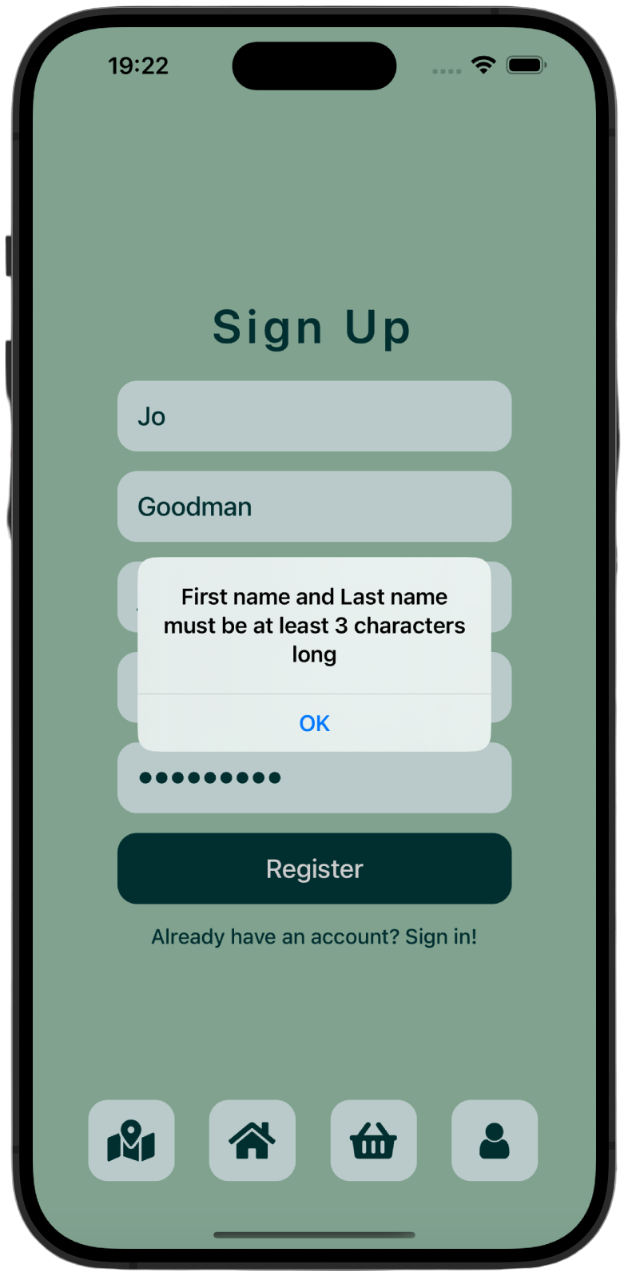
\includegraphics[width=0.3\textwidth]{images/front/register_invalid.png}
\end{center}

\subsection{Kategorie produktów}

Ekran kategorii stanowi pierwszy krok do przeglądania dostępnych produktów w wybranym sklepie. Centralnym elementem tego widoku jest siatka kategorii, umożliwiająca użytkownikowi intuicyjne poruszanie się po różnych grupach produktów. 

\begin{center} 
    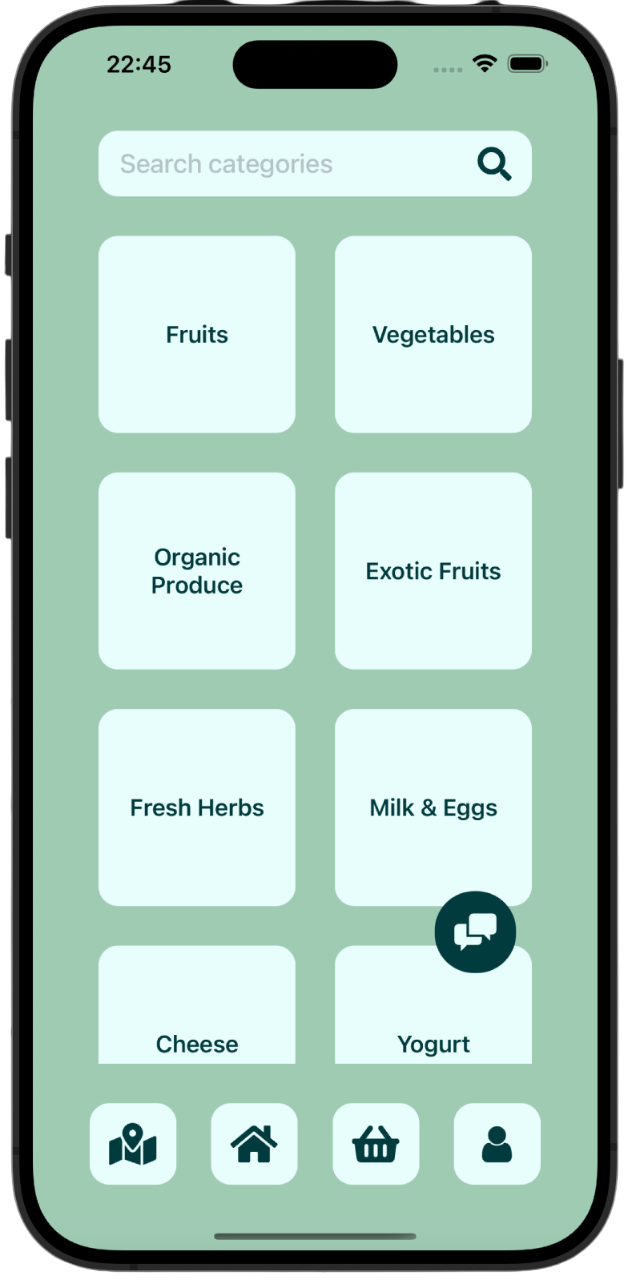
\includegraphics[width=0.3\textwidth]{images/front/categories_page.png} 
\end{center}

W górnej części widoku znajduje się pasek wyszukiwania, składający się z pola tekstowego oraz ikony lupy, umożliwiający szybkie filtrowanie kategorii na podstawie wprowadzonego tekstu. Wprowadzenie frazy w pole wyszukiwania automatycznie ogranicza widoczne wyniki, wyświetlając jedynie pasujące grupy produktów. Każdy kafelek siatki zawiera nazwę kategorii, a jego kliknięcie przekierowuje użytkownika do widoku produktów należących do wybranej kategorii. Siatkę można przewijać w pionie, aby odkrywać kolejne kafelki dostępne z listy. 

Dolną część ekranu zajmuje pasek nawigacyjny, który umożliwia szybki dostęp do innych kluczowych widoków aplikacji, takich jak mapa sklepów, profil użytkownika, koszyk oraz strona tytułowa. Widok zawiera również przeciągany dymek czatu, który pozwala na szybki kontakt z obsługą klienta. Jest on towarzyszem większości ekranów aplikacji, przez co został mu poświęcony osobny artykuł w sekcji o numerze \textit{x.x.x}.

\begin{center} 
    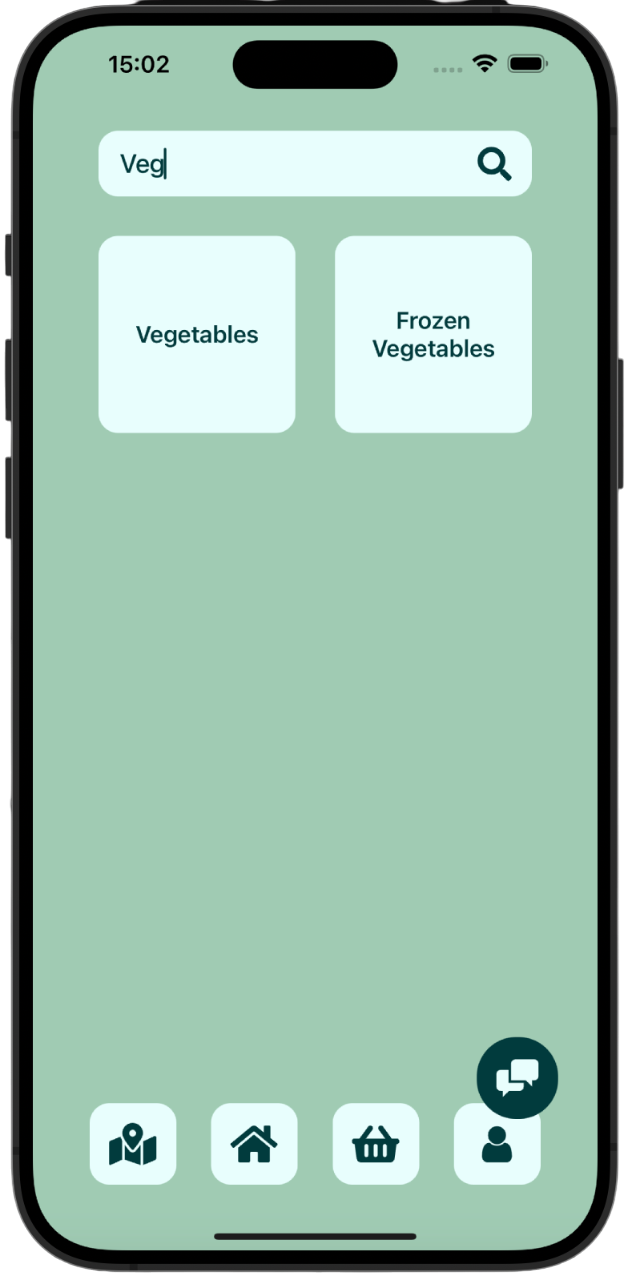
\includegraphics[width=0.3\textwidth]{images/front/categories_filtered.png} 
\end{center}

\subsection{Ekran produktów}

Ekran produktów pozwala użytkownikowi na przeglądanie i dodawanie do koszyka artykułów należących do wybranej kategorii. 

\begin{center} 
    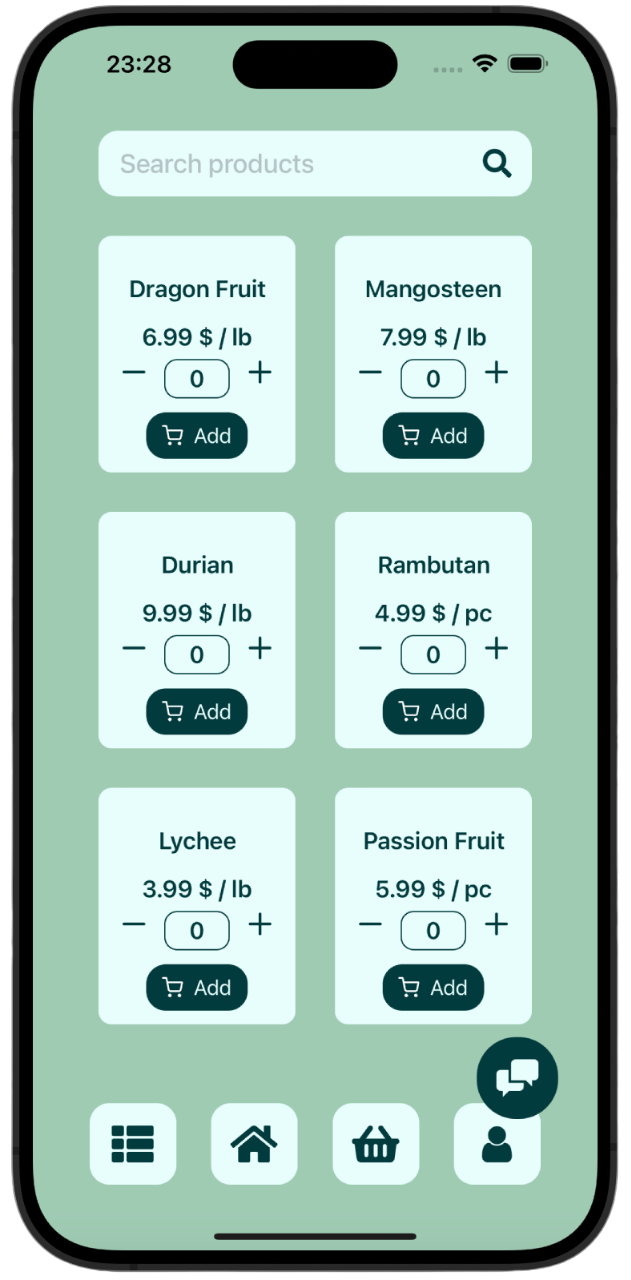
\includegraphics[width=0.3\textwidth]{images/front/products_page.png}  
\end{center}

Na samej górze widoku znajduje się pasek wyszukiwania, umożliwiający szybkie filtrowanie produktów po ich nazwie. Pasek zawiera pole tekstowe oraz ikonę lupy. Wprowadzenie tekstu w tym polu automatycznie zawęża widok, prezentując jedynie pasujące wyniki. Poniżej znajduje się przewijalna siatka produktów, w której każdy kafelek zawiera nazwę produktu, cenę oraz symbol jednostki miary. Dodatkowo dla każdego produktu dostępne są przyciski \textit{+} i \textit{–}, umożliwiające zwiększanie lub zmniejszanie ilości produktu, jaką użytkownik chce dodać do koszyka. Wartość wprowadzana przez kupującego jest automatycznie walidowana. Walidacja polega na sprawdzeniu, czy wprowadzony symbol jest liczbą całkowitą. Wartości mniejsze od zera nie są akceptowane. Pod każdym kafelkiem produktu znajduje się przycisk \textit{Add}, który dodaje wybraną ilość artykułu do koszyka gościa. Po naciśnięciu przycisku aplikacja odpowiednio weryfikuje możliwość dokonania zakupu poprzez sprawdzenie ilości produktu w magazynie. W przypadku błędnych danych, takich jak ilość większa niż dostępna, użytkownik otrzymuje odpowiedni komunikat w postaci alertu. 

Dół ekranu zdobi pasek nawigacyjny, który umożliwia powrót do ekranu kategorii, sprawdzenie stanu koszyka, przejście do profilu użytkownika czy strony głównej.

\begin{center} 
    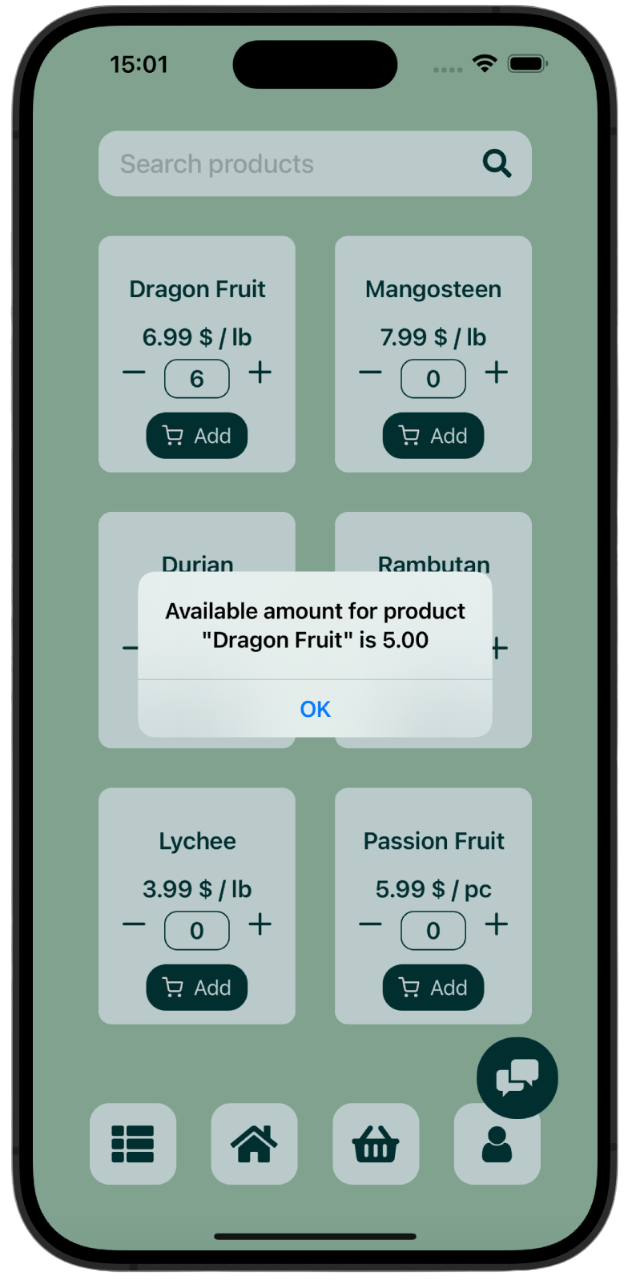
\includegraphics[width=0.3\textwidth]{images/front/products_amount.png}  
    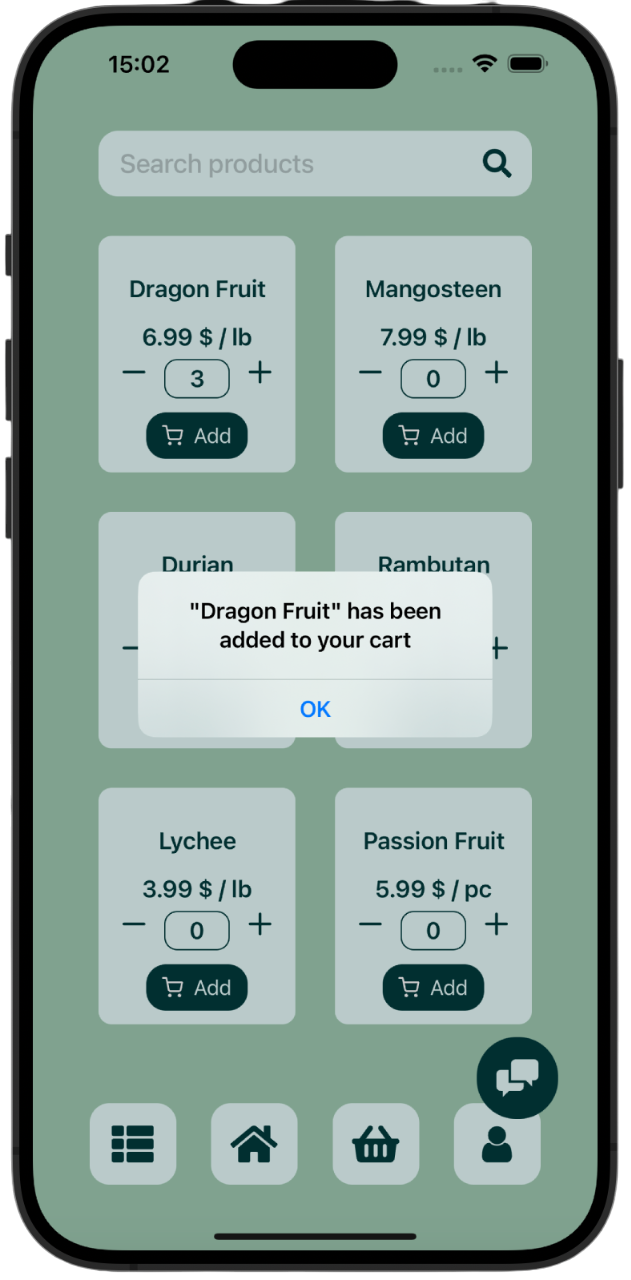
\includegraphics[width=0.3\textwidth]{images/front/products_added.png}  
\end{center}

\subsection{Koszyk użytkownika}

Ekran koszyka pozwala użytkownikowi zarządzać produktami dodanymi do koszyka oraz przygotować się do finalizacji zakupów. 

\begin{center}
    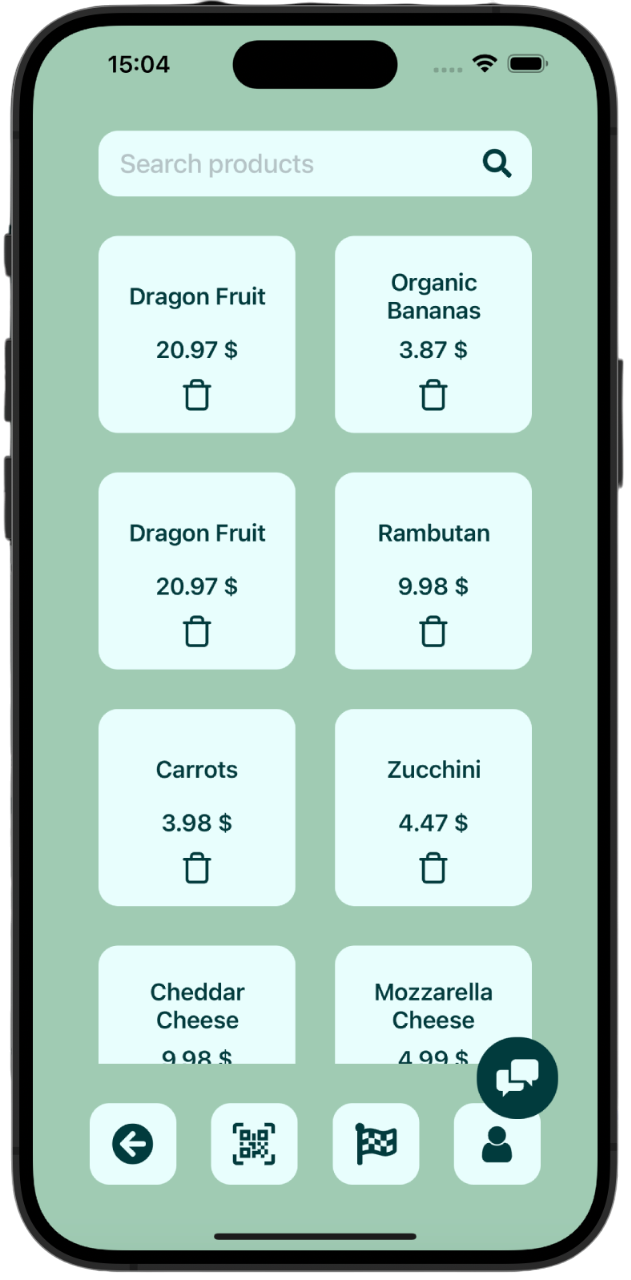
\includegraphics[width=0.3\textwidth]{images/front/cart_page.png}
\end{center}

W górnej części ekranu znajduje się pasek wyszukiwania, umożliwiający filtrowanie produktów według nazwy. Użytkownik może wprowadzić frazę w polu tekstowym, aby zawęzić listę wyświetlanych produktów, co znacznie ułatwia nawigację w przypadku dużej liczby elementów. Listę produktów w koszyku prezentuje przewijalna siatka, mieszcząca się pod paskiem wyszukiwania. Każdy element listy produktów w koszyku zawiera następujące informacje:
\begin{itemize}
    \item Nazwę produktu.
    \item Łączną cenę dla danej pozycji, obliczoną jako iloczyn ceny jednostkowej i ilości.
\end{itemize}

W przypadku chęci usunięcia produktu z koszyka, użytkownik posiada możliwość kliknięcia na ikonkę kosza na śmieci danego produktu. Aplikacja automatycznie aktualizuje widok koszyka po każdej zmianie.

Dolną część ekranu zajmuje pasek nawigacyjny, który umożliwia szybkie przejście do kolejnych widoków aplikacji. Należą do nich: generowanie kodu QR, mapa nawigująca po sklepie, profil użytkownika oraz powrót do poprzedniego ekranu.

\begin{center}
    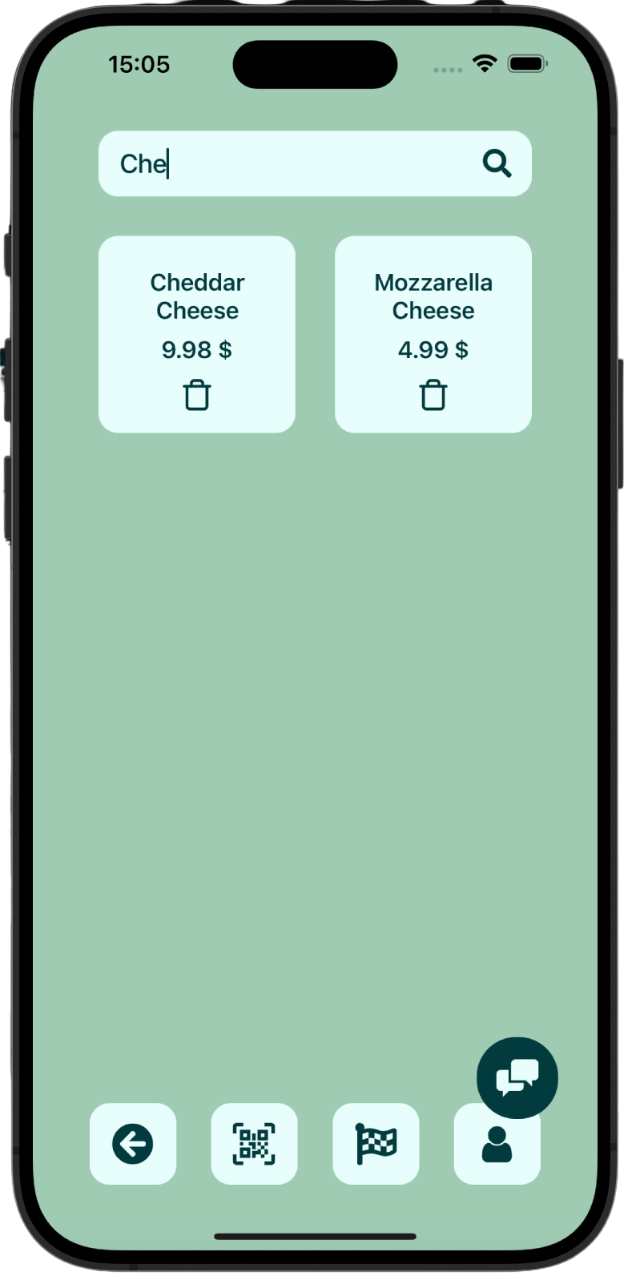
\includegraphics[width=0.3\textwidth]{images/front/cart_filtered.png}
\end{center}


\subsection{Generowanie kodu QR}

Po przejściu na ten ekran, pobierana jest lista produktów z koszyka danego kupującego. Dane na temat produktów zostają zawarte w wygenerowanym kodzie, który wyświetla się na środku ekranu po załadowaniu listy. W przypadku, gdy koszyk jest pusty, wyświetlany jest komunikat zachęcający do jego uzupełnienia. 

\begin{center}
    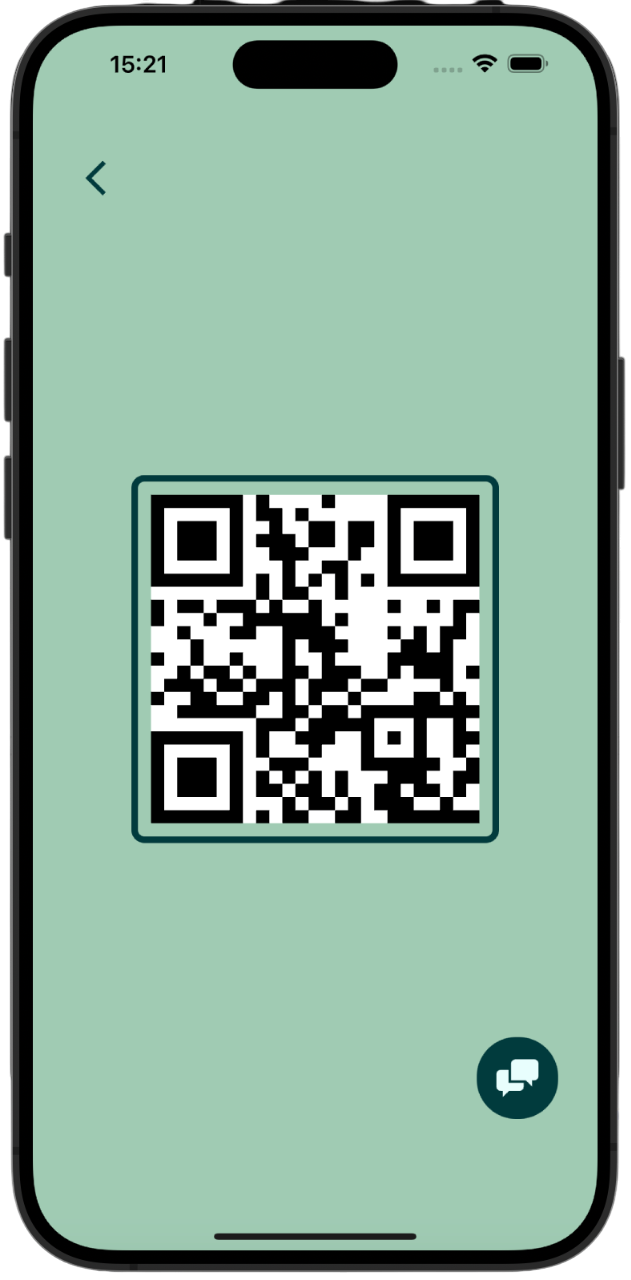
\includegraphics[width=0.3\textwidth]{images/front/qr_page.png}
\end{center}

Użytkownik ma możliwość zeskanowania kodu QR za pomocą czytnika danego sklepu, co pozwala na szybkie zinterowanie danych z aplikacją kasy samoobsługowej i nabicia zakupów na paragon. Za integrację kodu ze swoją aplikacją odpowiedzialny jest sam sklep. 

Aby wyjść z ekranu, należy nacisnąć symbol ptaszka, który przenosi użytkownika z powrotem do ekranu produktów.

\begin{center}
    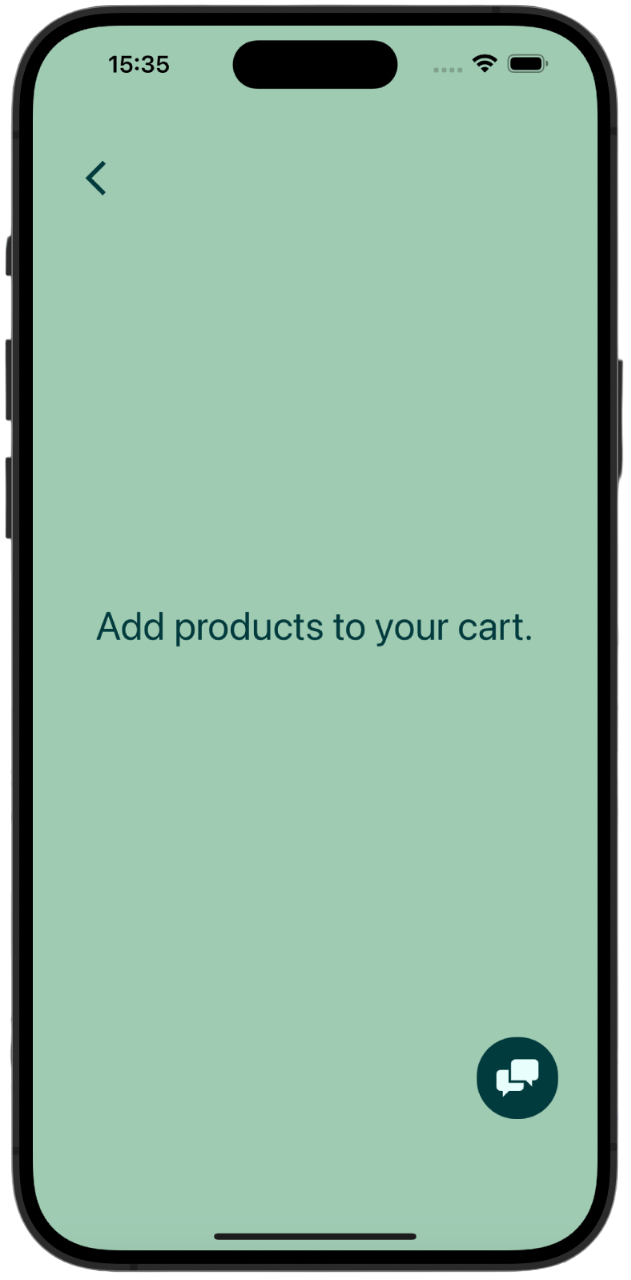
\includegraphics[width=0.3\textwidth]{images/front/qr_empty.png}
\end{center}

\subsection{Mapa sklepów}

Ekran wyboru sklepu pozwala użytkownikowi w intuicyjny sposób wybrać lokalizację sklepu, w którym planuje zrobić zakupy. Głównym elementem, pokrywającym cały widok jest interaktywna mapa, na której zaznaczone są wszystkie dostępne sklepy w formie markerów. Użytkownik może dowolnie przesuwać mapę oraz przybliżać i oddalać widok, aby lepiej zapoznać się z rozmieszczeniem sklepów. 

\begin{center}
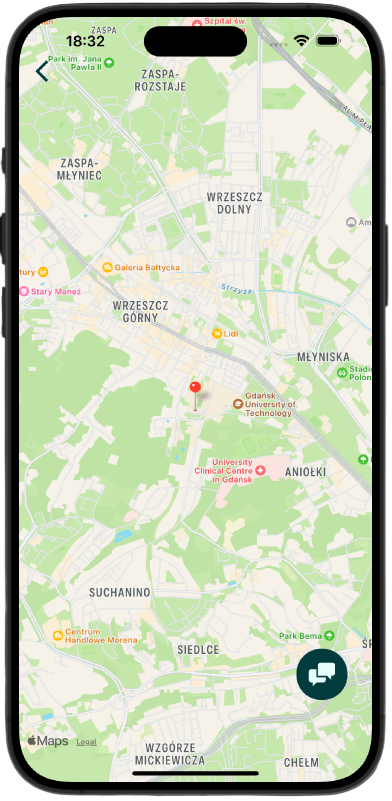
\includegraphics[width=0.3\textwidth]{images/front/store_page.png}
\end{center}

Punkt początkowy został ustawiony na sklep \textit{ETI PG} na potrzebę prezentacji. Kliknięcie na marker sklepu wyświetla szczegóły wybranej lokalizacji w dolnym panelu ekranu. Panel ten prezentuje nazwę sklepu oraz przycisk \textit{Select store}, który pozwala na potwierdzenie wyboru. Wybór sklepu jest sygnalizowany wyświetleniem komunikatu informującego o poprawnym zapisaniu decyzji. Dzięki temu użytkownik ma pewność, że jego wybór został zarejestrowany i aplikacja poprawnie zapisała ID sklepu, z którego należy pobrać kategorie i produkty.

W górnym lewym rogu ekranu znajduje się przycisk powrotu, który umożliwia szybkie przejście do poprzedniego widoku. 

\begin{center}
    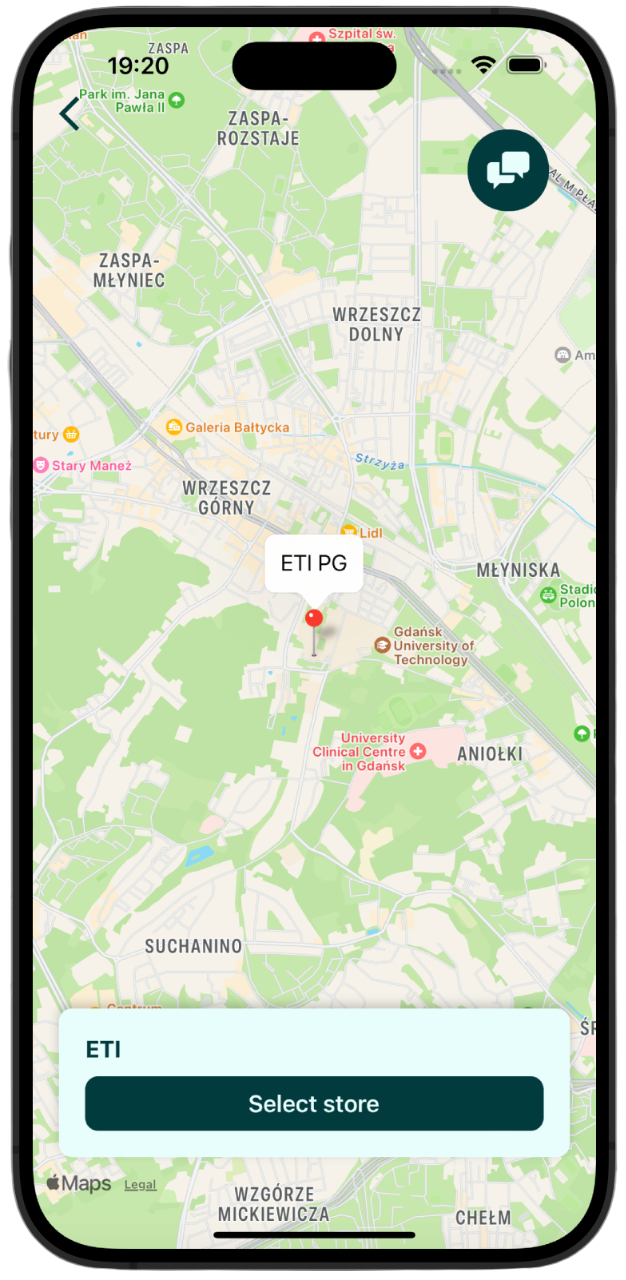
\includegraphics[width=0.3\textwidth]{images/front/store_selected.png}
    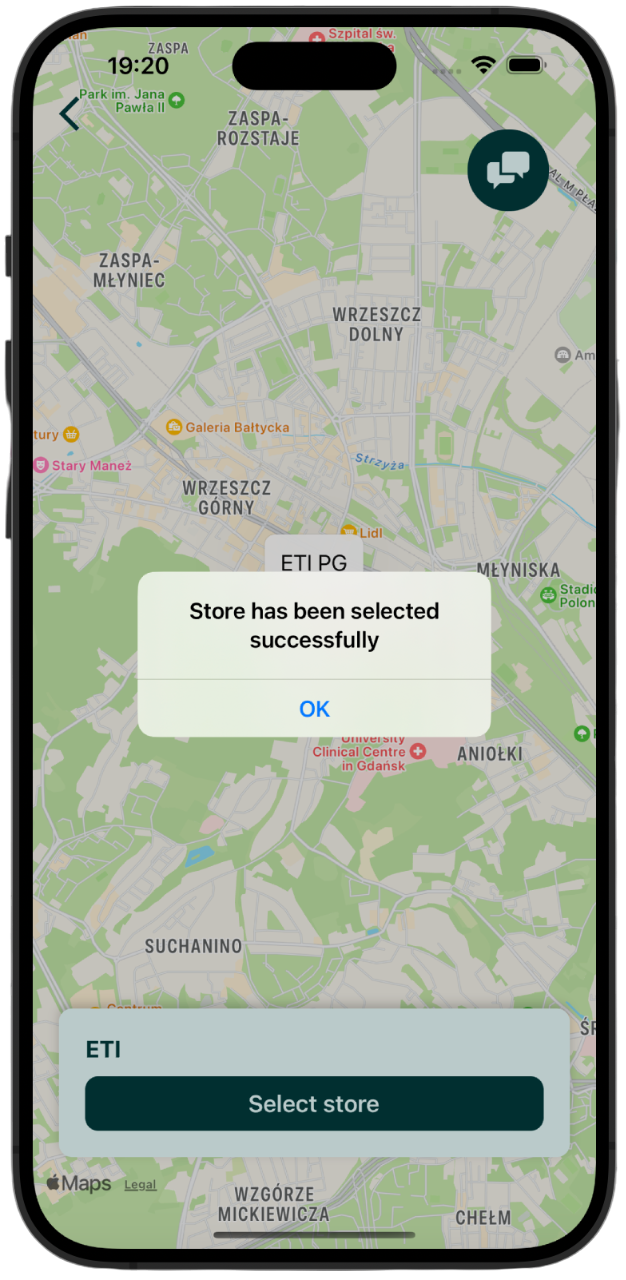
\includegraphics[width=0.3\textwidth]{images/front/store_success.png}
\end{center}


\subsection{Ekran nawigacji}

Ekran ten pozwala użytkownikowi na łatwe nawigowanie po sklepie, w celu zrealizowania zakupów w jak najkrótszym czasie. Jest to kluczowy widok, który odpowiada za podświetlenie klientowi trasy, jaką należy pokonać, aby uzyskać ten efekt.

\begin{center}
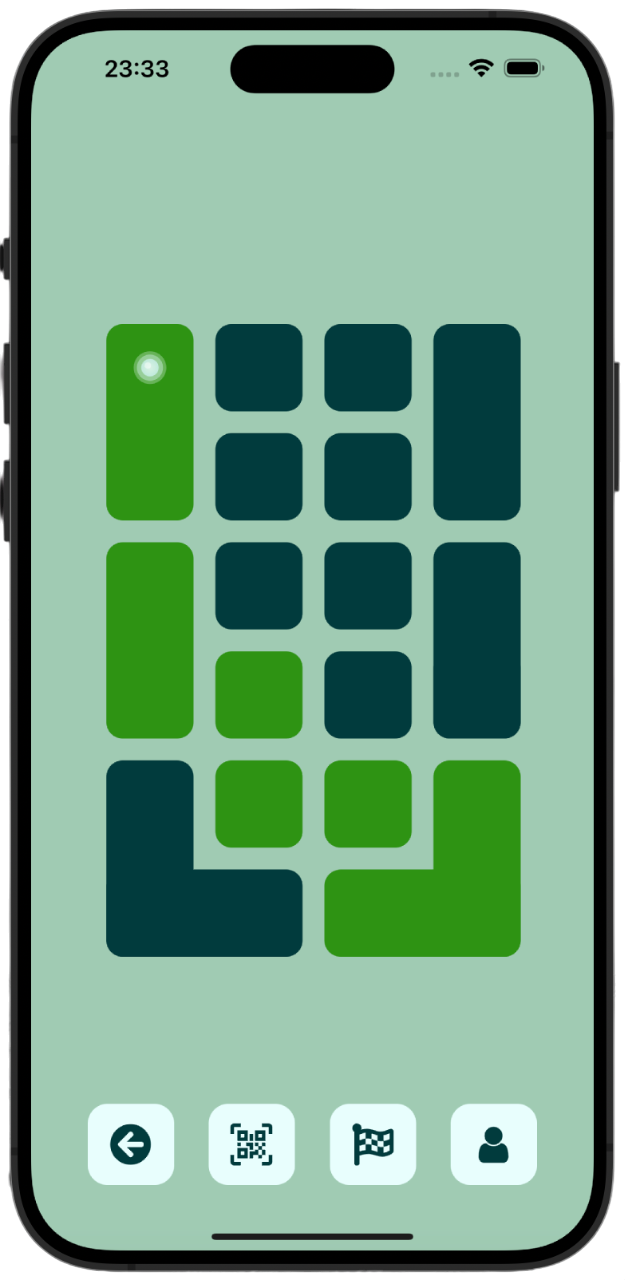
\includegraphics[width=0.3\textwidth]{images/front/navigation_page.png}
\end{center}

Ekran w znacznej większości składa się mapy sklepu, wygenerowanej ręcznie za pomocą grafiki SVG. Grafika ta, jest tworzona po wcześniejszej konsultacji ze sklepem. Podczas wejścia na ekran, aplikacja pobiera listę produktów z koszyka i na jej podstawie, wyznacza najkrótszą trasę, w postaci sektorów, które należy przebyć. Kolor trasy zmienia się na zielony, podczas gdy reszta sekcji pozostaje morska. Następnie za pomocą rozmieszczonych nadajników BLE, zostaje określone położenie użytkownika, które jest aktulizowane w czasie rzeczywistym, w postaci pulsującej, białej kropki.

Nawigacja w każdej chwili może zostać przerwana, chociażby poprzez powrót do koszyka, aby dodać kolejne produkty. W takim przypadku, po powrocie na ekran nawigacji, kupujący widzi nowo wygenerowaną trasę. Sam algorytm wyznaczania najkrótszej trasy, obsługa nadajników i pozycjonowanie eksploatatora zostaną omówione w osobnym rodziale.

Widok ten zawiera również pasek nawigacyjny, umożliwiający przejście do innych widoków, takich jak koszyk, profil kupującego czy generowanie kodu QR.

\begin{center}
    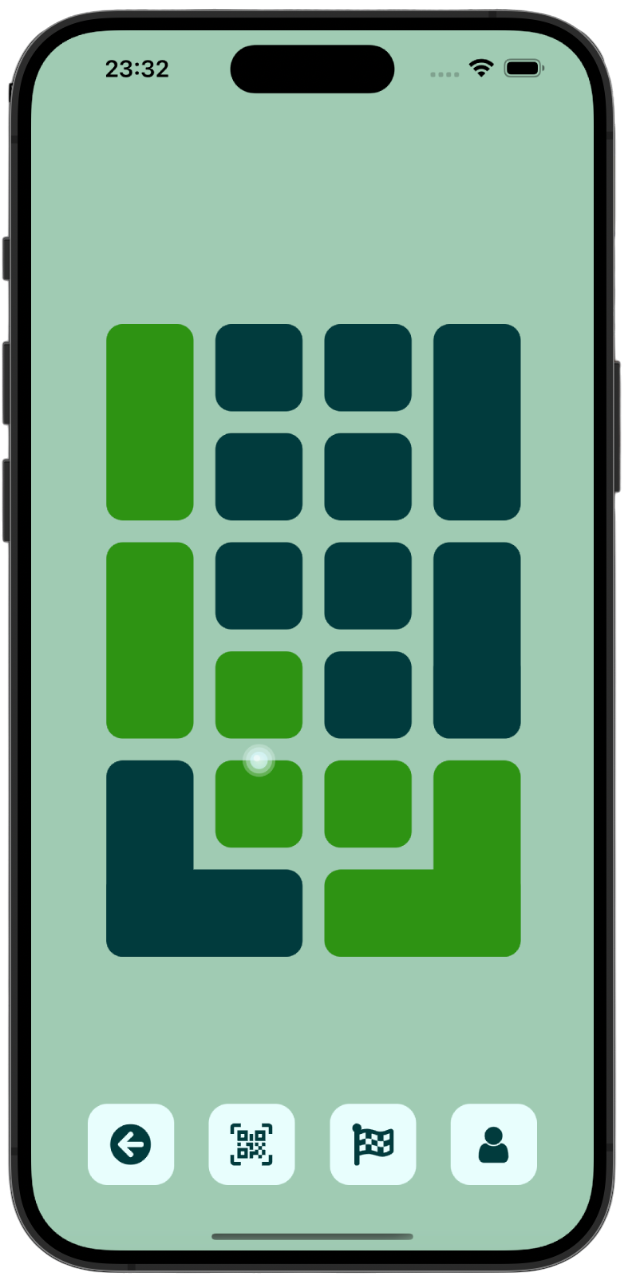
\includegraphics[width=0.3\textwidth]{images/front/navigation_moved.png}
\end{center}

\subsection{Profil użytkownika}

Ekran użytkownika umożliwia interakcję z chatbotem oraz zarządzanie kontem użytkownika, w tym możliwość wylogowania się z aplikacji.

\begin{center}
    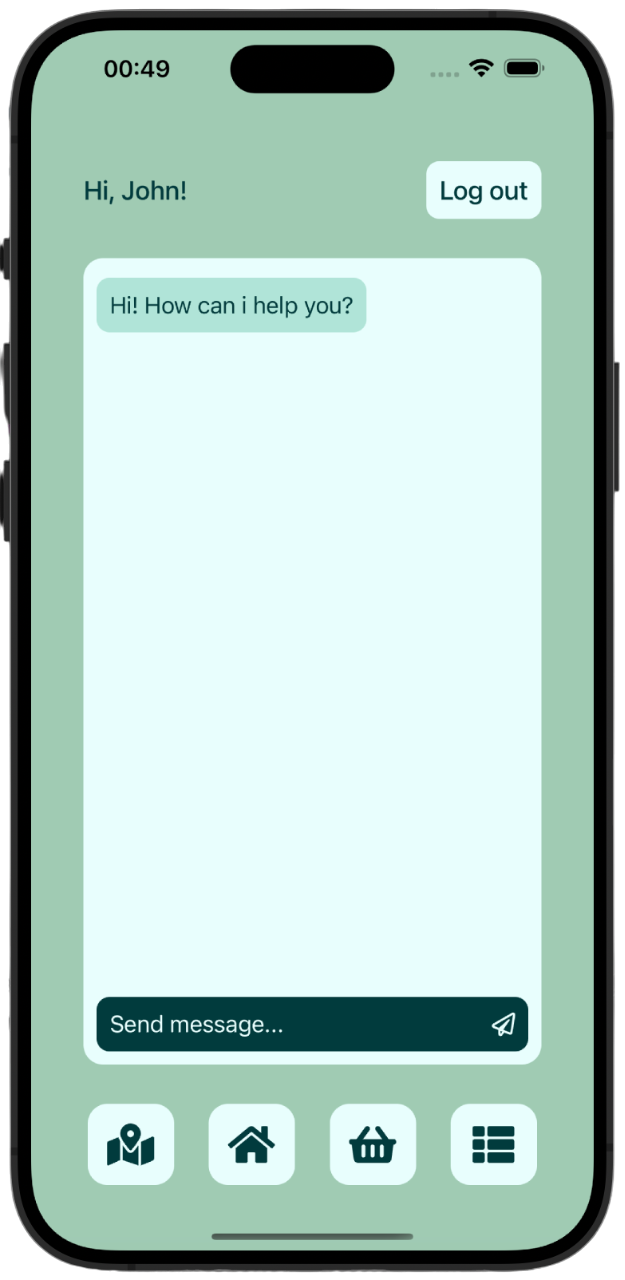
\includegraphics[width=0.3\textwidth]{images/front/user_page.png}
\end{center}

Na górze ekranu znajduje się powitanie użytkownika, wyświetlające jego imię, które jest pobierane z lokalnej pamięci aplikacji, aktualizowanej podczas poprawnego logowania. Obok powitania znajduje się przycisk \textit{Log out}, umożliwiający wylogowanie się z aplikacji i przekierowanie użytkownika na stronę główną. Wraz z kliknięciem tego przycisku czyszczona jest pamięć podręczna aplikacji, co skutkuje przerwaniem sesji i koniecznością ponownego zalogowania.

Główną część ekranu zajmuje chatbot, który pozwala na interakcję z użytkownikiem. Działa on w identyczny sposób, co wspomniany we wcześniejszych sekcjach dymek chatu, stąd zostanie on omówiony w osobnym rozdziale.

Dolną część ekranu zajmuje pasek nawigacyjny, który umożliwia przejście do innych sekcji aplikacji. Należą do nich: mapa sklepów, kategorie produktów, koszyk oraz strona tytułowa.

\section{Asystent AI}

\subsection{Profil użytkownika}

Na widoku użytkownika kluczowym elementem jest czat z botem, zaprojektowany w sposób intuicyjny i interaktywny. Po otwarciu widoku użytkownik widzi przestrzeń rozmowy, gdzie może prowadzić dialog z botem. Na starcie bot wysyła wiadomość powitalną, dostosowaną do użytkownika, np. \emph{"Hi! How can I help you?"}.  

\begin{center}
    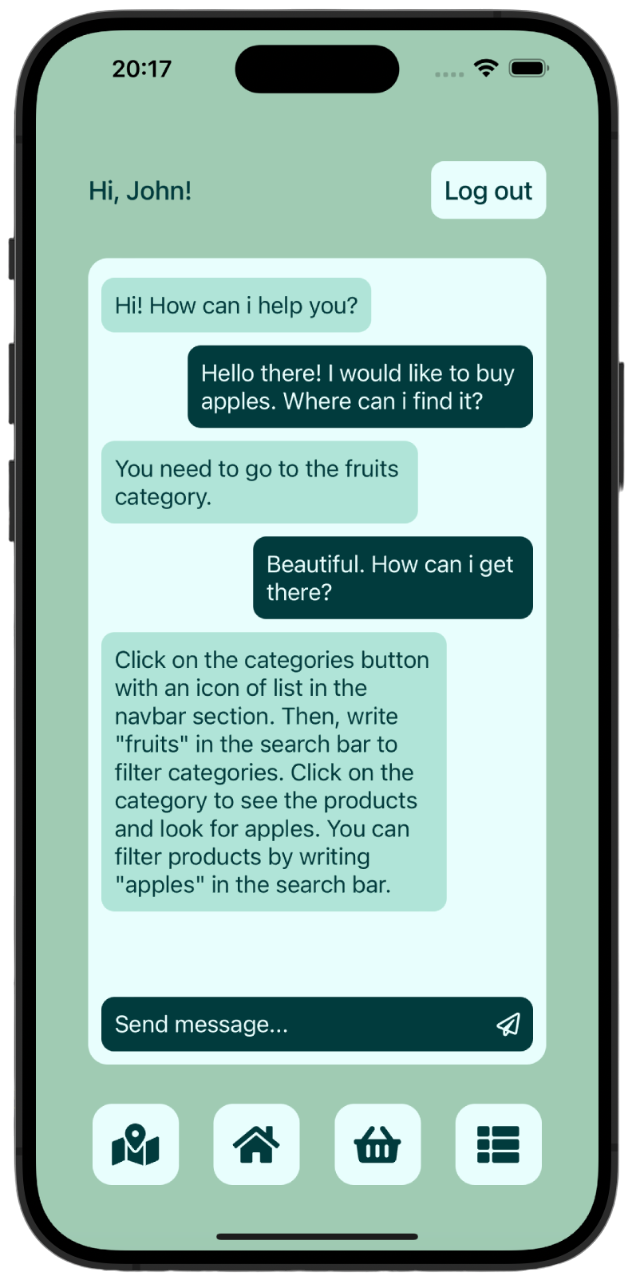
\includegraphics[width=0.3\textwidth]{images/front/user_chat.png}
\end{center}

Użytkownik wprowadza swoje pytania za pomocą pola tekstowego, a odpowiedzi bota pojawiają się dynamicznie w historii czatu. Bot potrafi odpowiadać na pytania dzięki dostępowi do bazy danych, która zawiera informacje o dostępnych sklepach, ich kategoriach, produktach oraz funkcjonalnościach aplikacji. Jeśli bot znajdzie odpowiednią informację, udziela konkretnej odpowiedzi lub wskazówek. Przykładowo:  

\begin{itemize}
    \item \emph{"Where is the nearest Biedronka?"} – bot podaje lokalizację najbliższego sklepu.  
    \item \emph{"I need milk."} – bot wskazuje najbliższy sklep, gdzie mleko jest dostępne.  
    \item \emph{"Where can I buy bread?"} – bot sugeruje sklepy w okolicy, które oferują pieczywo.  
\end{itemize}  

Jeśli jednak bot napotka bardziej złożone pytanie lub nie znajdzie odpowiedzi w bazie danych, wyświetla humorystyczną wiadomość, np. \emph{"I'm sorry. I don't understand."}, informując użytkownika o braku odpowiednich informacji.  

Bot jest w stanie odpowiedzieć na pytania dotyczące:  
\begin{itemize}
    \item Lokalizacji i szczegółów sklepów w okolicy,  
    \item Kategorii produktów i ich dostępności w określonych sklepach,  
    \item Funkcjonalności aplikacji, takich jak dodawanie produktów do koszyka czy używanie mapy do wyboru sklepów.  
\end{itemize}  

\begin{center}
    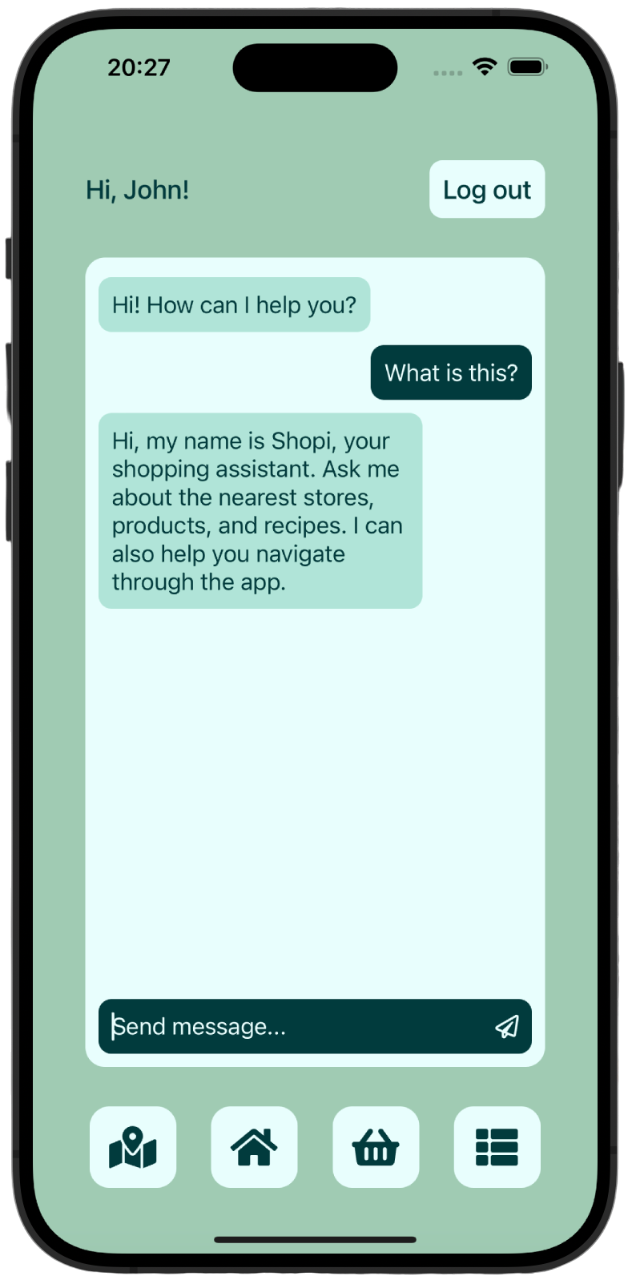
\includegraphics[width=0.3\textwidth]{images/front/what.png}
\end{center}

\subsection{Komponent dymka chatu}

\begin{center}
    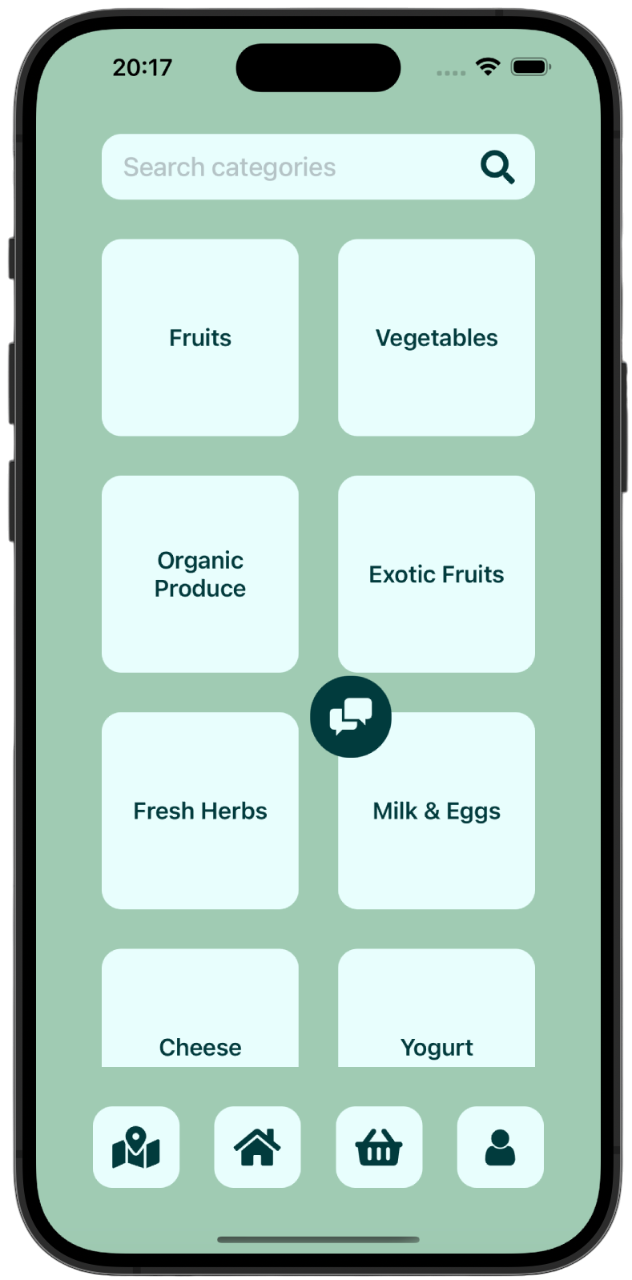
\includegraphics[width=0.3\textwidth]{images/front/cat_chat.png}
\end{center}

W przypadku korzystania z dymka chatu należy postępować analogicznie. Różnica polega na tym, że dymek jest widoczny na większości widoków w postaci małego, przeciąganego kółeczka z ikonką chatu. Po jego kliknięciu pojawia się niewielkie okno, w którym odbywa się rozmowa z asystentem - przebiega ona w identyczny sposób, co na ekranie kupującego. 


\begin{center}
    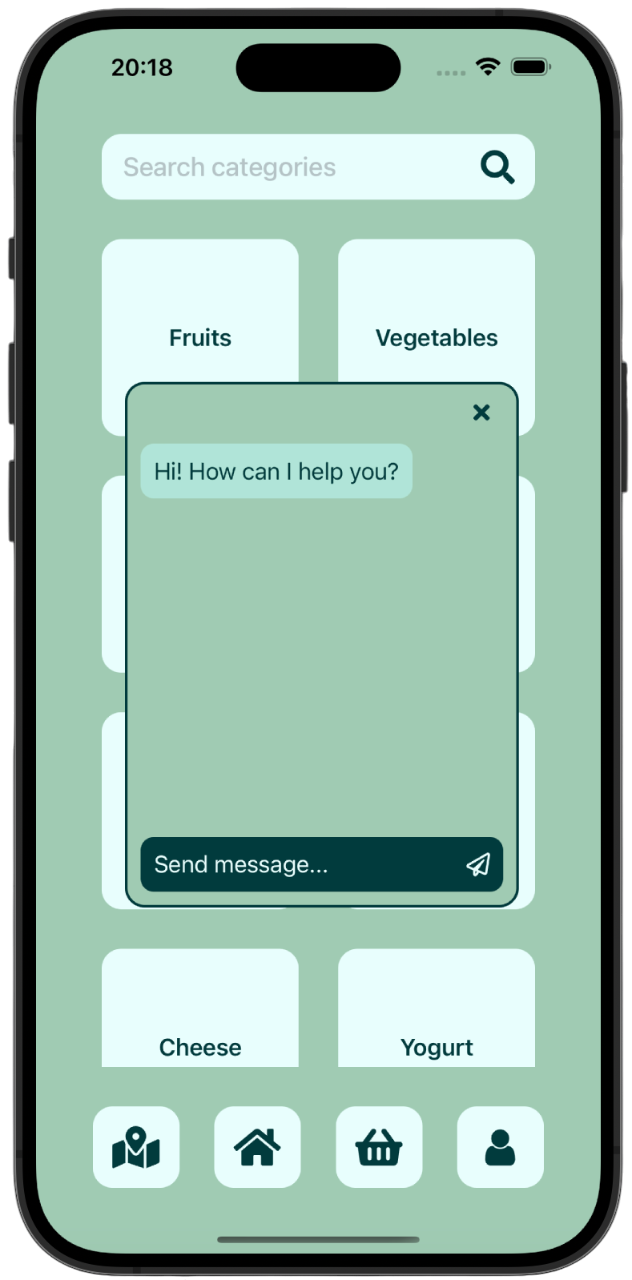
\includegraphics[width=0.3\textwidth]{images/front/cat_chat_open.png}
\end{center}

\section{Obsługa osoby niewidomej}

\subsection{Wprowadzenie}

Aplikacja \textit{Shopper} została zaprojektowana z myślą o użytkownikach niewidomych, umożliwiając im  korzystanie z jej funkcji za pomocą komend głosowych. Każdy ekran posiada odpowiednie drzewko zdarzeń, które prowadzi użytkownika przez kolejne kroki. Komendy są odczytywane na bieżąco, a kupujący otrzymuje wyraźne komunikaty informujące o dostępnych opcjach.

Aplikacja rozpoznaje wydawane polecenia, reaguje na ciszę oraz nieprawidłowe komendy, umożliwiając użytkownikowi efektywną interakcję.

\subsection{Strona tytułowa}

\subsubsection{Opis Ekranu}
Ekran startowy wita użytkownika i przedstawia podstawowe informacje o aplikacji. Proces nawigacji głosowej rozpoczyna się od komunikatu powitalnego i prowadzi użytkownika przez kolejne kroki.

\subsubsection{Przebieg Interakcji}
Po uruchomieniu aplikacji użytkownik zostaje przywitany komunikatem \textit{"Welcome to the Shopper app. You are currently on the start screen."}. Następnie aplikacja prosi użytkownika o wypowiedzenie komendy \textbf{start}, odtwarzając komunikat \textit{"Say 'start' to begin."}.

Jeśli użytkownik wypowie komendę \textbf{start}, aplikacja potwierdzi akcję komunikatem \textit{"Got it, moving forward."} i przejdzie do kolejnego ekranu. W zależności od statusu użytkownika, aplikacja przeniesie go:

\begin{itemize}
    \item Na \textbf{Ekran profilu}, jeśli użytkownik jest zalogowany.
    \item Na \textbf{Ekran logowania}, jeśli użytkownik nie jest zalogowany.
\end{itemize}

W sytuacji, gdy użytkownik wypowie nieznaną komendę, aplikacja poinformuje go o dostępnych opcjach komunikatem \textit{"Unknown command. The available option is: 'start'."} i ponownie będzie oczekiwać poprawnej odpowiedzi. Jeśli użytkownik nie odpowie, aplikacja zachęci go do powtórzenia komendy komunikatem \textit{"I did not hear you. Please repeat."}.

\subsection{Ekran logowania}

\subsubsection{Opis Ekranu}
Ekran logowania umożliwia użytkownikowi zalogowanie się do aplikacji za pomocą adresu e-mail oraz hasła. Proces nawigacji głosowej prowadzi użytkownika przez kolejne etapy logowania, od podania danych logowania po ewentualne błędy.

\subsubsection{Przebieg Interakcji}
Po przejściu na ekran logowania, aplikacja wita użytkownika komunikatem \textit{"Welcome to the login screen. Please say 'email' to enter your email address or 'register' to create a new account."}.

\begin{itemize}
    \item Jeśli użytkownik wypowie komendę \textbf{email}, aplikacja prosi o podanie adresu e-mail, odtwarzając komunikat \textit{"Please provide your email address."}.
    \item Jeśli użytkownik wypowie komendę \textbf{register}, zostanie przeniesiony do ekranu rejestracji, wraz z komunikatem \textit{"Moving to register."}.
\end{itemize}

Po wypowiedzeniu adresu e-mail, aplikacja powtarza go dla potwierdzenia komunikatem \textit{"I understood: [email]. Is that correct? Say 'yes' or 'no'."}.

\begin{itemize}
    \item Jeśli użytkownik odpowie \textbf{yes}, aplikacja przechodzi do etapu podania hasła, odtwarzając komunikat \textit{"Provide your password."}.
    \item Jeśli użytkownik odpowie \textbf{no}, aplikacja ponownie prosi o podanie adresu e-mail, odtwarzając komunikat \textit{"Please provide your email address again."}.
\end{itemize}

Po podaniu hasła, aplikacja prosi użytkownika o potwierdzenie: \textit{"I understood: [password]. Is that correct? Is that correct? Say 'yes' or 'no'."}.

\begin{itemize}
    \item Jeśli użytkownik odpowie \textbf{yes}, aplikacja sprawdza poprawność danych logowania, odtwarzając komunikat \textit{"Attempting to log you in."}. Jeśli dane są poprawne, użytkownik zostaje zalogowany, a aplikacja przekierowuje go na \textbf{Ekran kategorii}, odtwarzając komunikat \textit{"Login successful. Redirecting to categories page."}.
    \item Jeśli dane logowania są niepoprawne, aplikacja odtwarza komunikat \textit{"Login failed. Let's try again."} i wraca do etapu podania e-maila.
\end{itemize}


W sytuacji, gdy użytkownik wypowie nieznaną komendę lub zamilknie, aplikacja poinformuje go o dostępnych opcjach na danym etapie drzewka np poprze wypowiedzenie frazy \textit{"I did not hear you."} i powrócenia do etapu pobierania komendy.

\subsection{Rejestracja użytkownika}

\subsubsection{Opis Ekranu}

Ekran rejestracji umożliwia użytkownikowi utworzenie nowego konta w aplikacji poprzez podanie niezbędnych danych, takich jak imię, nazwisko, adres e-mail, hasło oraz potwierdzenie hasła. Ekran obsługuje nawigację głosową, która prowadzi użytkownika przez poszczególne kroki rejestracji.

\subsubsection{Przebieg Interakcji}

Po przejściu na ekran rejestracji, aplikacja wita użytkownika komunikatem: 
\textit{"You are on the register panel. Say 'register' to sign up or 'login' to go back to the sign in page."}.

\begin{itemize}
    \item Jeśli użytkownik wypowie komendę \textbf{register}, aplikacja przechodzi do kolejnych kroków rejestracji, zaczynając od pytania o imię.
    \item Jeśli użytkownik wypowie komendę \textbf{login}, to powróci do ekranu logowania.
\end{itemize}

Po wybranje komendzie rejestraci, aplikacja zaczyna wypełnianie formularza od imienia kupującego. Ważnym aspektem jest sygnalizowanie przez asystenta warunków jakie musi spełnić formularz: \textit{"Please provide your first name at least 3 characters long."}. 

Po wypowiedzeniu imienia aplikacja pyta o potwierdzenie:
\textit{"I understood: [firstname]. Is that correct? Say 'yes' or 'no'."}

\begin{itemize}
    \item Jeśli użytkownik odpowie \textbf{yes}, przechodzi do podania nazwiska.
    \item Jeśli odpowiedź to \textbf{no}, użytkownik jest proszony o ponowne podanie imienia.
\end{itemize}

Po podaniu nazwiska, aplikacja prosi o jego potwierdzenie, odtwarzając komunikat:
\textit{"I understood: [lastname]. Is that correct? Say 'yes' or 'no'."}

\begin{itemize}
    \item Jeśli użytkownik odpowie \textbf{yes}, aplikacja przechodzi do podania adresu e-mail: textit{"Please provide a valid email address."}.
    \item Jeśli odpowiedź to \textbf{no}, użytkownik jest proszony o ponowne podanie nazwiska.
\end{itemize}

Po wypowiedzeniu e-maila, aplikacja prosi o jego potwierdzenie:
\textit{"I understood: [email]. Is that correct? Say 'yes' if the email is correct, or 'no' to try again."}

\begin{itemize}
    \item Jeśli użytkownik odpowie \textbf{yes}, aplikacja przechodzi do podania hasła, mówiąc: \textit{"Provide your password at least 8 characters long."}.
    \item Jeśli odpowiedź to \textbf{no}, użytkownik jest proszony o ponowne podanie e-maila.
\end{itemize}.

Po wypowiedzeniu hasła, asystent pyta o jego potwierdzenie:
\textit{"I understood: [password]. Is that correct? Say 'yes' if the email is correct, or 'no' to try again.}
\begin{itemize}
    \item Jeśli użytkownik odpowie \textbf{yes}, aplikacja przechodzi do potwierdzenia hasła. Asystent odtwarza komunikat: \textit{"Please repeat your password."}.
    \item Jeśli odpowiedź to \textbf{no}, użytkownik jest proszony o ponowne podanie hasła.
\end{itemize}


Po potwierdzeniu wczytanego hasła, aplikacja waliduje dane, informując o tym kupującego za sprawą zdania \textit{"Attempting to sign you up."}.

\begin{itemize}
    \item W przypadku sukcesu aplikacja przenosi użytkownika na \textbf{Ekran kategorii produktów}, odtwarzając komunikat \textit{"Registration successful. Redirecting to login screen."}.
    \item W przeciwnym razie aplikacja wyświetla komunikat o błędzie: \textit{"Registration failed. Remember that Firstname and Lastname must be at least 3 characters long. Password must be at least 8 characters long. Email must be a valid email address. Let's try again."} i wraca do etapu pobierania imienia.
\end{itemize}

\subsection{Kategorie produktów}

\subsubsection{Opis Ekranu}

Ekran kategorii umożliwia użytkownikowi przeglądanie dostępnych kategorii produktów w wybranym sklepie. Użytkownik może przejść do konkretnej kategorii, wyszukiwać kategorie oraz nawigować do innych ekranów, takich jak mapa, koszyk czy profil kupującego.

\subsubsection{Przebieg Interakcji}
Po przejściu na ekran kategorii, aplikacja wita użytkownika komunikatem:  
\textit{"You are on the Categories screen."}

Następnie aplikacja przechodzi do listy dostępnych kategorii i odtwarza komunikat:  
\textit{"Say the name of a category to view its products or say 'Stores', 'Cart' or 'User' to visit other pages. Say 'categories' to get the categories list."}

W tym momencie użytkownik ma możliwość:

\begin{itemize}
    \item Wypowiedzenia nazwy jednej z kategorii, co przeniesie go do ekranu produktów w tej kategorii.  
    Na przykład, jeśli użytkownik powie \textbf{Electronics}, aplikacja odpowie:  
    \textit{"Moving to Electronics"} i przeniesie użytkownika do ekranu z produktami w tej kategorii, odtwarzając wiadomość: \textit{Moving to [nazwa kategorii]}
    \item Wypowiedzenia komendy \textbf{categories}, aby aplikacja odczytała dostępne kategorie. W odpowiedzi użytkownik usłyszy: \textit{"Available categories are: Electronics, Clothing, Books, Home Apliances..."}.
    \item Wypowiedzenia komendy \textbf{stors"}, co spowoduje przejście do ekranu mapy, z wiadomością \textit{"Moving to Stores"}.
    \item Wypowiedzenia komendy \textbf{cart"}, co przeniesie kupującego do ekranu koszyka, wraz z komunikatem \textit{"Moving to Cart"}.
    \item Wypowiedzenia komendy \textbf{user}, co przekieruje użytkownika do jego profilu, sygnalizując: \textit{"Moving to User"}.
\end{itemize}

Jeśli użytkownik wypowie komendę, której aplikacja nie rozumie, usłyszy:  
\textit{"I did not understand your command."}, a aplikacja wróci do listy dostępnych komend.

\subsection{Ekran produktów}

\subsubsection{Opis Ekranu}
Ekran produktów pozwala użytkownikowi na przeglądanie dostępnych produktów, wybieranie ich ilości oraz dodawanie ich do koszyka. Użytkownik może również nawigować do innych widoków aplikacji, takich jak kategorie, koszyk czy ekran użytkownika. Wszystkie akcje są wspierane przez system nawigacji głosowej, który prowadzi użytkownika krok po kroku.

\subsubsection{Przebieg Interakcji}
Po wejściu na ekran produktów aplikacja wita użytkownika komunikatem: \textit{"You are on the Products screen."} Następnie informuje o dostępnych opcjach: \textit{"Say the name of a product and give its quantity to add it to the Cart. Call 'Stores', 'Cart' or 'User' to visit other pages. You can check the products list by saying 'products'."}

Jeśli użytkownik wypowie komendę \textbf{products}, aplikacja odtwarza listę dostępnych produktów, na przykład: \textit{"Available products are: apples, bananas, oranges."} Po zakończeniu odczytywania lista zostaje zamknięta, a aplikacja ponownie przypomina użytkownikowi o możliwych komendach.

Kiedy użytkownik zdecyduje się dodać produkt do koszyka, może wypowiedzieć jego nazwę, na przykład \textbf{"apples"}. W odpowiedzi aplikacja prosi o określenie ilości z podaną jednostką, za pomocą komunikatu: \textit{"Please provide the quantity of apples in kilograms or say 'no' to cancel."} Jeśli użytkownik poda liczbę, na przykład \textbf{"two"}, aplikacja potwierdza zrozumienie: \textit{"I understood: 2 apples. Is that correct? Say 'yes' or 'no'."}

Jeśli użytkownik odpowie \textbf{yes}, produkt zostaje dodany do koszyka, a aplikacja informuje o sukcesie: \textit{"Added 2 apples to the cart. Returning to the product list."} Jeśli natomiast użytkownik odpowie \textbf{no}, aplikacja ponownie prosi o określenie ilości: \textit{"Please provide the quantity of apples in kilograms or say 'no' to cancel."}

W przypadku podania ilości przekraczającej dostępny stan magazynowy, aplikacja odpowiada komunikatem: \textit{"There is only [quantity] apples left. Please try again."} W takim przypadku użytkownik musi określić mniejszą ilość.

Po zakończeniu dodawania produktów użytkownik może nawigować do innych widoków aplikacji. Na przykład, wypowiadając \textbf{"categories"}, aplikacja odtwarza komunikat: \textit{"Moving to Categories"} i przekierowuje użytkownika na ekran kategorii. Wypowiedzenie \textbf{"cart"} powoduje przejście na ekran koszyka z komunikatem: \textit{"Moving to Cart"}, a komenda \textbf{"user"} przenosi na ekran użytkownika z komunikatem: \textit{"Moving to User"}.

W przypadku, gdy użytkownik wypowie nieznaną komendę, aplikacja informuje o błędzie: \textit{"I did not understand your command."} i przypomina dostępne opcje. Jeśli użytkownik nie odpowie, aplikacja zachęca go do działania komunikatem: \textit{"I did not hear you. Please repeat."} W ten sposób ekran produktów pozostaje prosty i intuicyjny, pozwalając użytkownikowi na wygodne zarządzanie produktami za pomocą głosu.

\subsection{Koszyk użytkownika}

\subsubsection{Opis Ekranu}
Ekran koszyka umożliwia użytkownikowi przeglądanie produktów dodanych do koszyka oraz zarządzanie ich zawartością. Użytkownik może usuwać wybrane produkty, przeglądać pełną listę produktów w koszyku, a także przejść do innych widoków aplikacji. Nawigacja głosowa wspiera użytkownika w każdym kroku.

\subsubsection{Przebieg Interakcji}
Po wejściu na ekran koszyka aplikacja wita użytkownika komunikatem: \textit{"You are on the Cart screen."} Następnie informuje o dostępnych opcjach: \textit{"Say 'products' to get the full content of your cart. Say the name of a product to delete it. You can visit other pages by saying 'Categories', 'Code', 'Navigation', or 'User'."}

Jeśli użytkownik wypowie komendę \textbf{products}, aplikacja odczytuje listę produktów znajdujących się w koszyku, na przykład: \textit{"Products in your cart: apples, bananas, oranges."} Po zakończeniu komunikat kończy się przypomnieniem dostępnych opcji, aby użytkownik mógł podjąć kolejne działania.

W przypadku, gdy użytkownik wypowie nazwę produktu, na przykład \textbf{"apples"}, aplikacja odtwarza komunikat potwierdzający: \textit{"Product apples has been deleted from cart."} i usuwa produkt z koszyka. Po tej akcji użytkownik wraca do głównego menu koszyka, a aplikacja przypomina dostępne komendy.

Jeżeli użytkownik zdecyduje się przejść do innego widoku, może wypowiedzieć jedną z dostępnych komend. Na przykład, komenda \textbf{"categories"} powoduje przejście na ekran kategorii z komunikatem: \textit{"Moving to Categories."} Podobnie, komenda \textbf{"code"} przenosi użytkownika do widoku generowania kodu z informacją: \textit{"Moving to Code."}, natomiast \textbf{"navigation"} lub \textbf{"user"} przenoszą odpowiednio na widok nawigacji lub użytkownika.

W przypadku, gdy użytkownik wypowie nieznaną komendę, aplikacja odtwarza komunikat: \textit{"I did not understand your command."} i powtarza dostępne opcje, zachęcając użytkownika do spróbowania ponownie. Jeśli użytkownik pozostanie cichy, aplikacja przypomni się komunikatem: \textit{"I did not hear your response."}, co pomaga utrzymać płynność interakcji.

\subsection{Generowanie kodu QR}

\subsubsection{Opis Ekranu}
Ekran generowania kodu QR umożliwia użytkownikowi wygenerowanie kodu QR na podstawie aktualnej zawartości koszyka. Kod QR zawiera wszystkie informacje o produktach w koszyku, co pozwala na łatwe przekazanie tych danych do innych systemów lub urządzeń. Po przejściu na ten ekran aplikacja automatycznie pobiera produkty z koszyka i generuje odpowiedni kod QR, po czym wyświetla go na ekranie.

\subsubsection{Przebieg Interakcji}
Po wejściu na ekran generowania kodu QR aplikacja wita użytkownika komunikatem: \textit{"You are on the Code screen."}. Następnie informuje o dostępnych opcjach: \textit{"Say 'back', to go back to the cart."}

Jeżeli użytkownik wypowie komendę \textbf{back}, aplikacja odtwarza komunikat: \textit{"Moving to Cart."} i przekierowuje użytkownika z powrotem na ekran koszyka, gdzie może on ponownie zarządzać zawartością koszyka.

W przypadku, gdy użytkownik wypowie nieznaną komendę, aplikacja odtwarza komunikat: \textit{"I did not understand your command."} i ponownie przedstawia dostępne opcje, aby pomóc użytkownikowi w nawigacji. Jeśli użytkownik nie odpowie, aplikacja przypomni się komunikatem: \textit{"I did not hear your response."}, zachęcając go do wypowiedzenia polecenia.


\subsection{Mapa sklepów}

\subsubsection{Opis Ekranu}
Ekran mapy sklepów umożliwia użytkownikowi wybór sklepu z dostępnej listy. W momencie przejścia na ten ekran aplikacja pobiera listę sklepów z bazy danych i prezentuje je w formie mapy oraz listy interaktywnych komend głosowych. Po wybraniu sklepu użytkownik jest automatycznie przenoszony do kategorii, gdzie może kontynuować zakupy.

\subsubsection{Przebieg Interakcji}
Po wejściu na ekran mapy sklepów aplikacja wita użytkownika komunikatem: \textit{"You are on the Stores screen."} Następnie informuje o dostępnych opcjach: \textit{"Say the name of a store to select it or 'back', to go back to categories. Say 'stores' to get the full list of stores."}

Jeżeli użytkownik wypowie nazwę sklepu, aplikacja odpowiada komunikatem potwierdzającym: \textit{"Store [nazwa sklepu] has been successfully selected."} Wybrany sklep zostaje zapisany jako aktywny w pamięci podręcznej aplikacji, a użytkownik jest automatycznie przekierowywany na ekran kategorii.

Jeśli użytkownik chce poznać pełną listę dostępnych sklepów, może wypowiedzieć komendę \textbf{stores}, na co aplikacja odpowie wiadomością zawierającą wszystkie dostępne sklepy, np.: \textit{"Available stores are: Store A, Store B, Store C"} — lista jest generowana dynamicznie w oparciu o dane z bazy danych.

W przypadku, gdy użytkownik chce wrócić do poprzedniego widoku, wystarczy powiedzieć \textbf{back}, a aplikacja przeniesie go na ekran kategorii, komunikując: \textit{"Moving to Categories."}

Jeżeli użytkownik wypowie nieznaną komendę, aplikacja odtworzy komunikat: \textit{"I did not understand your command."} i ponownie wyświetli dostępne opcje. W przypadku braku odpowiedzi użytkownika aplikacja przypomni się wiadomością: \textit{"I did not hear your response."}, zachęcając do podjęcia akcji.

\subsection{Profil użytkownika}

\subsubsection{Opis Ekranu}
Ekran profilu użytkownika zapewnia dostęp do podstawowych funkcji zarządzania kontem, takich jak wylogowanie, oraz umożliwia nawigację do innych kluczowych widoków aplikacji: kategorii, koszyka i mapy sklepów. Jest to punkt centralny dla użytkownika, który chce zarządzać swoim doświadczeniem w aplikacji. Posiada on również chat z asystentem AI, jednak ta funkcja nie jest obsługiwana w trybie głosowym.

\subsubsection{Przebieg Interakcji}
Po wejściu na ekran profilu użytkownika aplikacja wita go komunikatem: \textit{"You are on the User screen."} Następnie przedstawia dostępne opcje: \textit{"Say 'Log out' to log out of your account. Say 'Categories', 'Cart' or 'Stores', to visit other pages."}

Jeśli użytkownik zdecyduje się wylogować, wypowiadając \textbf{log out}, aplikacja natychmiast odpowiada: \textit{"You have been logged out."} i wykonuje akcję wylogowania, co skutkuje usunięciem danych sesji i powrotem do ekranu logowania lub strony startowej.

Aby przejść do innych sekcji aplikacji, naley wybrać jedną z dostępnych komend:
\begin{itemize}
    \item \textbf{categories} — przenosi użytkownika na ekran kategorii, z komunikatem: \textit{"Moving to categories."}
    \item \textbf{cart} — przenosi użytkownika na ekran koszyka, z komunikatem: \textit{"Moving to cart."}
    \item \textbf{stores} — przenosi użytkownika na ekran mapy sklepów, z komunikatem: \textit{"Moving to stores."}
\end{itemize}
